% !TEX program = pdflatex
% Scholarly research formulation: thermally induced deformation and conjugate heat
% transfer in a channel with two-way thermoelastic coupling.
% Compile: pdflatex -> bibtex -> pdflatex -> pdflatex
\documentclass[11pt,a4paper]{report}

\usepackage[margin=2.4cm]{geometry}
\usepackage{amsmath,amssymb}
\usepackage{booktabs,longtable,array}
\usepackage[table]{xcolor}
\usepackage{siunitx}
\usepackage{tikz}
\usetikzlibrary{arrows.meta,positioning}
\usepackage{caption}
\captionsetup{labelfont=bf,labelsep=period}
\usepackage{graphicx}
\usepackage[numbers,sort&compress]{natbib}
\usepackage[hidelinks,pdftitle={Thermally induced deformation and conjugate heat transfer in a channel},pdfauthor={Research formulation document}]{hyperref}

% status macros used ONLY in the consolidated evidence tables of Appendix B
\newcommand{\VER}{\textcolor{green!50!black}{\textbf{verified}}}
\newcommand{\VWC}{\textcolor{blue!60!black}{\textbf{verified with conditions}}}
\newcommand{\INC}{\textcolor{red!70!black}{\textbf{superseded (incorrect)}}}
\newcommand{\UNR}{\textcolor{orange!80!black}{\textbf{unresolved}}}

% short macros
\newcommand{\eps}{\varepsilon}
\newcommand{\bn}{\mathbf{n}}
\newcommand{\bu}{\mathbf{u}}
\newcommand{\bd}{\mathbf{d}}
\newcommand{\bsig}{\boldsymbol{\sigma}}
\newcommand{\beps}{\boldsymbol{\eps}}
\newcommand{\bI}{\mathbf{I}}
\newcommand{\tr}{\operatorname{tr}}
\newcommand{\Om}{\Omega}
\newcommand{\Ga}{\Gamma}

\title{\textbf{Thermally induced deformation and conjugate heat transfer in a
channel with two-way thermoelastic coupling}\\[6pt]
\large Mathematical formulation, reconciled analytical development, and verification plan\\[4pt]
\normalsize Pre-implementation research document ---
\emph{International Journal of Numerical Methods for Heat \& Fluid Flow} (target venue)}
\author{}
\date{Version of 18 October 2026}

\begin{document}
\maketitle

\begin{abstract}
\noindent
A mathematical formulation is developed for steady conjugate heat transfer in a two-dimensional
channel whose upper wall contains a finite thermoelastic segment heated on its outer face. Heat
conduction through the wall establishes a through-thickness temperature gradient; the associated
thermal eigen-curvature deflects the segment into the flow passage; the deformed passage modifies
the velocity and temperature fields; and the resulting interfacial heat flux closes the coupling
back onto the wall temperature. The model couples incompressible laminar flow, advection--diffusion
heat transfer, steady conduction, and linear isotropic thermoelasticity under plane strain, with
traction and heat-flux continuity imposed on a common deformed interface, the wall equation being
carried to the pinned beam--column form at finite membrane force. The plane-strain
constitutive reduction, mean-stress identity, free thermal curvature, support-dependent bowing and
thermal-buckling limits, and the pressure-datum-consistent relative magnitude of hydraulic and
thermally driven deflection are derived explicitly for the present configuration. A baseline
operating point is evaluated from first principles, the governing dimensionless groups are
identified from the equations on a single characteristic-length basis, and a conforming-mesh
finite-element formulation with streamline-stabilized transport and a deformed-domain fixed-point
iteration is proposed together with a verification hierarchy based on analytical solutions and
published benchmark data. The document distinguishes established theory, analytical results derived
for this configuration, and quantities that can only be obtained from the future computations; no
simulation results are reported. Discrepancies identified and reconciled during preparation of the formulation --- each with its
resolution basis, and the few items that remain explicitly unresolved --- together with the
conditions gating coupled production computations, are collected in the appendices and in the
accompanying audit archive.
\end{abstract}

\tableofcontents

\chapter{Introduction and physical motivation}
\label{ch:intro}

\section{Problem statement}
Consider steady laminar forced convection in a two-dimensional slit channel. A finite segment of the
upper wall is not rigid: it consists of a thin thermoelastic layer whose outer face is heated by a
uniformly applied heat flux, as realised, for example, by a film heater. Conduction across the layer
produces a through-thickness temperature difference whose magnitude is governed by the wall
conductivity and thickness. Linear thermoelasticity associates with this gradient a free thermal
curvature; with the segment ends pinned, the segment bows toward the interior of the passage. The
resulting displacement redistributes the flow cross-section, alters the near-wall velocity and
temperature gradients, and therefore changes the interfacial convective heat flux. That flux, in
turn, is one of the boundary data of the conduction problem in the wall. The wall temperature, the
deformation, and the fluid thermal field are thus coupled in both directions, and a consistent
solution requires their simultaneous determination.

The present document formulates this coupled problem mathematically, derives the reduction implied
by plane strain and by the thin-wall geometry, evaluates a baseline operating point analytically,
and specifies a numerical formulation and a verification hierarchy for its eventual computation. No
simulation results are reported; the distinction between established theory, results derived here
for this configuration, and quantities that remain to be computed is maintained throughout.

\section{Physical motivation}
Wall-guided micro heat exchangers and microreactors are increasingly fabricated from polymers and
polymer composites, which combine low thermal conductivity with a comparatively high coefficient of
thermal expansion. For the same imposed heat flux, such walls sustain through-thickness temperature
drops orders of magnitude larger than metallic walls of equal thickness, and their free thermal
curvature is correspondingly larger (the comparison is quantified in
Chapter~\ref{ch:baseline}). When the wall thickness is comparable to the channel height, the
associated deformation is not a perturbation of the passage geometry but a modification of it, and
heat-transfer predictions that assume a fixed geometry become geometry-dependent in a
thermally self-consistent way.

Deformation of flow passages by thermal loading is well known from thermoelastic-contact and
regenerative-cooling analyses, in which the deformation is typically computed a posteriori from a
frozen flow solution, i.e.\ in one direction of coupling. In the configuration considered here, the
deformation is itself the principal quantity of interest and feeds back on the convective boundary
condition that produces it. A number of natural modelling questions follow and motivate the present
work: under which combinations of wall material, geometry, and hydraulic operation is the thermal
bowing comparable to the channel height; what bounds does thermal buckling of the pinned segment
impose on admissible heating; how does the interaction behave under imposed flow rate relative to
imposed pressure drop; and how large are the residual stresses carried by the wall.

\section{Scope of the present study}
The analysis is confined to a two-dimensional geometry, steady state, laminar incompressible flow,
and linear isotropic thermoelasticity under plane strain, with the wall equation extended to the
pinned beam--column form at finite membrane force. The baseline treats imposed heat flux on
the outer face of the deformable segment; a variant with imposed outer-face temperature is retained
as a separately documented operating regime. The solid is modelled by two-dimensional elasticity and
steady conduction; the reduced wall equations are used for design estimates
and benchmark comparisons. Buoyancy is disposed of at the baseline by a length-consistent
Richardson-number estimate (three orders of magnitude below the mixed-convection range), with a
regime guard that re-opens the question should a parameter study drive the number upward, as
discussed in Chapters~\ref{ch:baseline} and~\ref{ch:limitations}.

Transient coupling, mesh dynamics, and the associated discrete geometric conservation-law
requirements \cite{lesoinne1996geometric} are outside the present scope and are recorded as the
conditions of a possible start-up study. Likewise, creep of the polymer wall, manufacturing
tolerances, and contact resistance at the interface are excluded from the baseline and are listed
among the model limitations.

\section{Relation to existing work}
Fluid--structure interaction with heat transfer has been studied for cavity and channel geometries
in which the deformation is driven by fluid traction \cite{soti2015steady,alsabery2019numerical,%
saleh2025laminar}, and fully nonlinear thermo-fluid--structure interaction of flexible cantilevers
in a differentially heated cavity has been computed \cite{kumar2026thermo}.
In the configuration studied here, the deformation mechanism is instead the wall's own thermal
eigen-curvature, the flow is a confined forced-convection slit at moderate Reynolds number, and the
coupling closes through the conjugate thermal boundary condition. A detailed comparison, the
resulting positioning of the intended contribution, and the limits of that positioning imposed by
the available literature search are developed in Chapter~\ref{ch:contribution}.

\section{Organisation of the document}
Chapter~\ref{ch:model} fixes the geometry, assumptions, sign conventions, and material data.
Chapter~\ref{ch:equations} states the governing equations and the constitutive relations together
with the principles from which they follow. Chapter~\ref{ch:derivations} derives the plane-strain
reduction and the analytical relations used for design estimates. Chapter~\ref{ch:interface}
assembles the boundary and interface conditions. Chapter~\ref{ch:dimensionless} identifies the
dimensionless groups and the admissibility bounds of the regime. Chapter~\ref{ch:baseline}
evaluates the baseline operating point in full arithmetic detail. Chapter~\ref{ch:numerics}
proposes the finite-element formulation and solution procedure. Chapter~\ref{ch:validation}
specifies the verification and validation methodology. Chapter~\ref{ch:contribution} reviews the
related literature and states the proposed contribution and its bounds.
Chapter~\ref{ch:limitations} collects the limitations. Appendices contain the notation, the
arithmetic calculations in independently checkable cells, a dimensionless dictionary, and the audit
record (discrepancy register, consolidated evidence status, unresolved source checks, and the
conditions attached to the staged implementation decisions).

\chapter{Mathematical model and modelling assumptions}
\label{ch:model}

\section{Geometry and reference configuration}
\label{sec:domains}

The configuration is two-dimensional. Reference coordinates $X=(X,Y)$ label material points of the
solid and the undeformed fluid domain. The fluid reference domain,
$\Om_f^0=\{(X,Y):-L_e\le X\le L+L_o,\;0\le Y\le H_0\}$,
consists of a rigid entrance section $\Om_e=(X\in[-L_e,0])$, a section $\Om_d=(X\in[0,L])$ facing
the deformable wall, and a rigid exit section $\Om_o=(X\in[L,L+L_o])$, all of undeformed height
$H_0$. The only deformable body is the solid strip
$\Om_s^0=[0,L]\times[H_0,H_0+d]$
of thickness $d$ spanning the full out-of-plane depth. Its lower face $Y=H_0$ shares the fluid
boundary; its upper face $Y=H_0+d$ receives the imposed thermal load. The strip is embedded in a
rigid casing and is pinned at both ends, $X=0$ and $X=L$: the displacement vanishes there while the
bending moment vanishes (Assumption~A9). Figure~\ref{fig:geometry} shows the configuration,
Table~\ref{tab:geometry} records the design point.

\begin{figure}[t]
\centering
% fig_geometry.tex -- body content of Figure 1 (scaled layout, not to absolute scale)
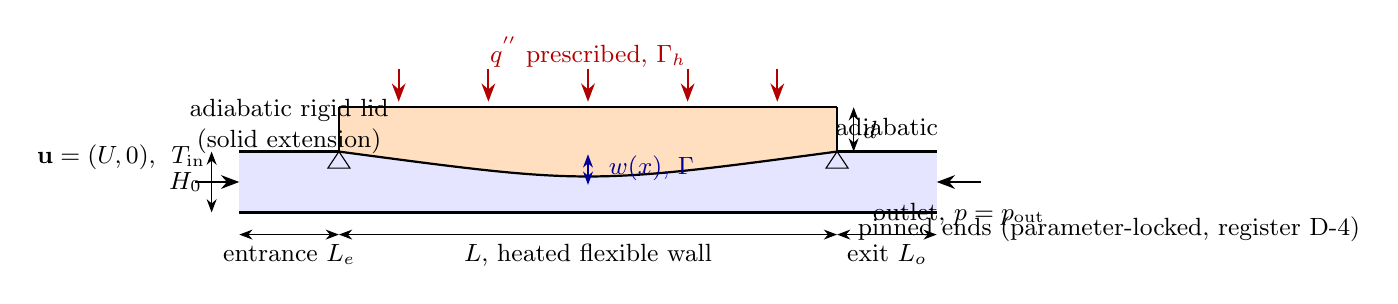
\begin{tikzpicture}[x=1pt,y=1pt,>=Stealth,font=\small]
% ---------------- geometry (points as described in caption) ----------------
\def\Le{36}\def\L{180}\def\Lo{36}          % entry, heated, exit (horizontal pts)
\def\Hf{22}                                 % channel height (exaggerated for readability)
\def\ds{16}                                 % wall thickness. origin of fluid at lower-left of entry zone
\coordinate (O) at (0,0);
% fluid channel
\fill[blue!10] (O) rectangle ++(\Le+\L+\Lo,\Hf);
\draw[thick] (0,0) -- ++(\Le+\L+\Lo,0);
\draw[thick] (0,\Hf) -- ++(\Le,0) coordinate (L1);
\draw[thick] (\Le+\L,\Hf) -- ++(\Lo,0);
% flexible wall strip (heated segment), deformed bow shown by parabola through points
\coordinate (A) at (\Le,\Hf);
\coordinate (B) at (\Le+\L,\Hf);
\coordinate (At) at (\Le,\Hf+\ds);
\coordinate (Bt) at (\Le+\L,\Hf+\ds);
\fill[orange!25] (At) -- (Bt) -- (B) .. controls (\Le+\L/2,\Hf-12) .. (A) -- cycle;
\draw[thick] (A) .. controls (\Le+\L/2,\Hf-12) .. (B);
\draw[thick] (At) -- (Bt);
\draw[thick] (A) -- (At); \draw[thick] (B) -- (Bt);
% heat flux arrows on top of heated wall
\foreach \x in {0.12,0.30,0.5,0.7,0.88}{
  \draw[->,red!70!black,thick] (\Le+\x*\L,\Hf+\ds+14) -- (\Le+\x*\L,\Hf+\ds+2);}
\node[red!70!black] at (\Le+\L/2,\Hf+\ds+20) {$q^{''}$ prescribed, $\Ga_h$};
% adiabatic labels
\node[align=center] at (\Le/2,\Hf+9) {adiabatic rigid lid\\(solid extension)};
\node[align=center] at (\Le+\L+\Lo/2,\Hf+9) {adiabatic};
% inlet/outlet arrows
\draw[->,thick] (-16,\Hf/2) -- (0,\Hf/2) node[midway,above left=1pt] {$\bu=(U,0)$,\; $T_\mathrm{in}$};
\draw[<-,thick] (\Le+\L+\Lo,\Hf/2) -- ++(16,0);
\node[below] at (\Le+\L+\Lo+8,\Hf/2-4) {outlet, $p=p_\mathrm{out}$};
% interface and wall-motion annotation
\draw[<->,blue!60!black] (\Le+\L/2,\Hf-12) -- (\Le+\L/2,\Hf-1);
\node[blue!60!black,anchor=west] at (\Le+\L/2+4,\Hf-6) {$w(x)$, $\Ga$};
% dimension lines
\draw[<->] (\Le,-8) -- ++(\L,0) node[midway,below] {$L$, heated flexible wall};
\draw[<->] (0,-8) -- ++(\Le,0) node[midway,below] {entrance $L_e$};
\draw[<->] (\Le+\L,-8) -- ++(\Lo,0) node[midway,below] {exit $L_o$};
\draw[<->] (-10,0) -- ++(0,\Hf) node[midway,left] {$H_0$};
\draw[<->] (\Le+\L+6,\Hf) -- ++(0,\ds) node[midway,right] {$d$};
% pinned supports
\foreach \p in {(A),(B)}{\draw \p -- ++(-4,-6) -- ++(8,0) -- cycle;}
\node[anchor=west] at (\Le+\L+4,-6) {pinned ends (parameter-locked, register D-4)};
\end{tikzpicture}

\caption{Configuration of the coupled problem (schematic, not to scale). Rigid entrance and exit
sections of the channel; a thermoelastic segment of length $L$ and thickness $d$, pinned at its
ends and heated on its outer face $\Ga_h^0$; the conjugate interface $\Ga_{\mathrm{if}}$ between
fluid and solid; a rigid, adiabatic lower wall. The interface deflection $w$ is measured positive
into the channel (Figure~\ref{fig:signs}).}
\label{fig:geometry}
\end{figure}

\begin{table}[t]
\centering\small
\caption{Geometry and operating point used as the baseline design. Values marked \emph{design} are
free choices of the study; the derived hydraulic diameter uses the slit value $D_h=2H_0$.}
\label{tab:geometry}
\begin{tabular}{p{4.0cm}p{1.7cm}p{4.2cm}p{2.6cm}}
\toprule
Quantity & Symbol & Value & Basis \\
\midrule
Channel height & $H_0$ & \SI{5.0e-4}{\metre} & design \\
Hydraulic diameter & $D_h=2H_0$ & \SI{1.0e-3}{\metre} & derived \\
Heated, deformable length & $L$ & \SI{3.0e-2}{\metre} & design \\
Entrance / exit lengths & $L_e,L_o$ & \SI{1.0e-2}{\metre}; \SI{2.0e-2}{\metre} & design \\
Wall thickness & $d$ & \SI{3.0e-3}{\metre} & design \\
Mean inlet velocity & $U$ & \SI{5.0e-2}{\metre\per\second} & design \\
Imposed heat flux (baseline regime) & $q^{''}$ & \SI{5.0e3}{\watt\per\square\metre} & design \\
Inlet and reference temperatures & $T_{\mathrm{in}},T_{\mathrm{ref}}$ & to be fixed at data freeze & temperature differences only enter \\
\bottomrule
\end{tabular}
\end{table}

The deformed interface is defined by the solid displacement field $\bd$ on the reference interface,
\begin{equation}
\Ga_{\mathrm{if}}=\{x=X+\bd(X):\;X\in[0,L]\times\{H_0\}\},
\end{equation}
and the steady fluid domain $\Om_f$ is obtained by extending the interface displacement into
$\Om_f^0$ through a mesh-extension map $\widehat{\mathbf w}$ specified in
Section~\ref{sec:ale}. The fluid equations are posed on $\Om_f$; the solid equations on the
reference configuration, consistent with small strains (Assumption~A4).

\section{Modelling assumptions}
\label{sec:assumptions}
Each assumption is stated with its justification and its range of validity; the quantitative checks
supporting the numerical bounds are carried out in Chapter~\ref{ch:baseline}.

\begin{itemize}\itemsep2pt
\item[\textbf{A1}] \emph{Two-dimensional geometry and plane strain.} The out-of-plane dimension is
large compared with $H_0$ and $d$, and loading is uniform along it, so the flow and temperature
fields are two-dimensional and the solid is in plane strain, $\eps_{zz}=0$. Plane strain, rather
than plane stress, is the closure appropriate to a wide bonded wall
\cite{boley1960theory,timoshenko1970elasticity}; its consequences for the constitutive reduction
are derived in Chapter~\ref{ch:derivations}.
\item[\textbf{A2}] \emph{Newtonian, constant-property fluid.} The working fluid is water at near-ambient
temperature, with constant density $\rho$, viscosity $\mu$, specific heat $c_p$, and conductivity
$k_f$. The self-consistency of constant properties is established a posteriori: the computed
fluid-side temperature excursions at baseline are of order $1$--$3$ K
(Section~\ref{sec:baselinecalc}), over which the property variation remains below a few per cent.
The influence of buoyancy is examined separately through the Richardson number
(Sections~\ref{sec:buoyancy-baseline}, \ref{sec:limitations}).
\item[\textbf{A3}] \emph{Homogeneous isotropic linear thermoelastic solid.} The wall is a PEEK-class
polymer with constant $E$, $\nu$, $\alpha$, $k_s$, $\rho_s$, $c_s$. Deviations (grade-to-grade
variability, mild anisotropy of extruded stock) are treated by the sensitivity requirements of
Chapter~\ref{ch:validation}; the numerical values used below are datasheet-representative and are
to be frozen against a specific datasheet before implementation (Appendix~B, item C-6).
\item[\textbf{A4}] \emph{Small strains, moderate rotations.} The strain measures must remain small:
the bending fibre strain, the arc-stretching membrane strain, and the total mechanical surface
strain. Linear kinematics alone is \emph{not} sufficient for the pinned, axially constrained strip,
because the thermal membrane force interacts with the transverse deflection at leading order; the
adopted kinematics is therefore the reduced (frozen-force) von K\'arm\'an beam--column level of
Section~\ref{sec:deriv:beamcolumn}, which reduces to the linear relation when the membrane force
is negligible. At the baseline the bending fibre strain is $9.9\times10^{-4}$, the
maximum total mechanical surface strain is $\approx5.4\times10^{-3}$, the arc-stretching term is
$\approx1.8\times10^{-4}$, and the maximum slope is $0.03$~rad
(Section~\ref{sec:baselinecalc}); all are far below the order-one failure limits of the
hypothesis. Geometric admissibility is expressed through these strain and slope measures together
with a mesh bound $|w|/H_0\le0.5$ with positive element Jacobians, rather than through a purely
geometric deflection ratio alone (Appendix~B, register D-11, D-15).
\item[\textbf{A5}] \emph{Steady flow and energy; quasi-static solid mechanics.} The structural wave
time across the wall is seven orders of magnitude shorter than the slowest transport time
(Section~\ref{sec:steadytimes}), so the mechanical problem is quasi-static and inertia is omitted
from \eqref{eq:equilibrium}.
\item[\textbf{A6}] \emph{Laminar flow.} The design keeps $\mathrm{Re}_{D_h}\le100$ (baseline value $50$),
well below the transition range for plane channels, which justifies \eqref{eq:momentum}.
\item[\textbf{A7}] \emph{Negligible viscous dissipation.} The Brinkman number at baseline is of order
$10^{-6}$ (Chapter~\ref{ch:baseline}); the dissipation term is retained as a re-inclusion option
with the rule stated at \eqref{eq:fluidenergy}.
\item[\textbf{A8}] \emph{Perfect thermal contact at the interface.} No contact resistance is included at
$\Ga_{\mathrm{if}}$; temperature and heat flux are continuous
(\eqref{eq:iftemp}--\eqref{eq:ifflux}).
\item[\textbf{A9}] \emph{Ideal pinned supports and rigid casing.} The strip ends have zero displacement,
zero applied moment, and zero heat flux; the surrounding casing is taken rigid and adiabatic, and
its interior pressure equals the outlet datum of condition~B2, which fixes the load reference of
Section~\ref{sec:deriv:pressure}. Implementation note: the pins are imposed on the full end edge
($X=0,L$), which differs from ideal point pins by Saint-Venant end layers of width $O(d)$; at the
baseline aspect ratio $L/d=10$ this contributes a few per cent of global stiffening, and a
one-time numerical check (full-edge versus corner pins) is part of the verification programme
(Chapter~\ref{ch:validation}).
\item[\textbf{A10}] \emph{Uniform imposed flux as the baseline thermal load (regime N).} A uniform
$q^{''}$ models a film heater and fixes the total heat input per unit depth, $Q'=q^{''}L$, which is
the quantity entering the global enthalpy balance (Section~\ref{sec:quality}). A second regime
(regime D, imposed outer-face temperature $T_h$) is retained as a separately labelled study;
comparisons across regimes are meaningful only at matched total heat input.
\end{itemize}

\section{Sign and traction conventions}
\label{sec:signs}
A single interface normal $\bn$ is used throughout, directed from the fluid into the solid.
Pressure on the wall is positive in compression; Cauchy stress in the solid is positive in tension.
The interface deflection is denoted $w$ and is measured \emph{from the reference interface into the
channel} (hence $w=-d_2$ in terms of the upward-positive solid displacement $d_2$). Wall curvature
is taken positive when the wall bows into the channel; within the small-slope assumption this gives
the design relation $\kappa=-w^{''}$, and a constant eigen-curvature $\kappa_{\mathrm{th}}>0$
produces $w=\kappa_{\mathrm{th}}x(L-x)/2\ge0$ (Section~\ref{sec:deriv:deflection}).
Fluid heat flux along $+\bn$ carries heat out of the fluid. Using one normal on both sides of the
traction equality is what renders the interface boundary terms in the weak statement of
Section~\ref{sec:coupling} exactly antisymmetric, so that they cancel in a monolithic assembly
without modelling error.

\begin{figure}[t]
\centering
% fig_signs.tex -- body content of Figure 2 (sign/traction conventions at the interface)
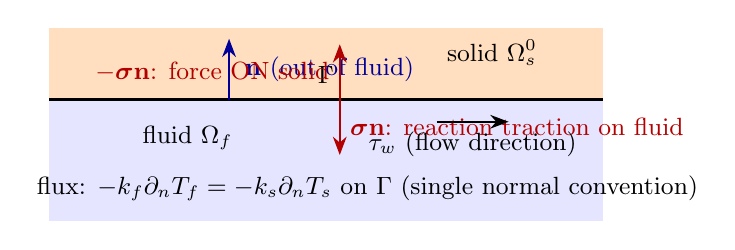
\begin{tikzpicture}[x=1pt,y=1pt,>=Stealth,font=\small]
% fluid (below) / solid (above) separated by interface
\fill[blue!10] (-10,-44) rectangle (190,0);
\fill[orange!25] (-10,0) rectangle (190,26);
\node at (40,-14) {fluid $\Om_f$};
\node at (150,17) {solid $\Om_s^{0}$};
% interface
\draw[very thick] (-10,0) -- (190,0) node[midway,above=2pt] {$\Ga$};
% normal convention: n points out of the fluid, i.e. up and into the solid
\draw[->,thick,blue!60!black] (55,0) -- ++(0,22) node[midway,right=2pt] {$\bn$ (out of fluid)};
% by (5.1) with the single normal n (out of fluid, into solid): the force ON the solid is
% -sigma_f n (pressure part +p n, pointing up, away from the fluid); sigma_f n is the reaction on the fluid
\draw[->,thick,red!70!black] (95,0) -- ++(0,20) node[midway,left] {$-\bsig\bn$: force ON solid};
\draw[->,thick,red!70!black] (95,0) -- ++(0,-20) node[midway,right] {$\bsig\bn$: reaction traction on fluid};
% wall shear sense
\draw[->,thick] (130,-8) -- ++(26,0) node[midway,below] {$\tau_w$ (flow direction)};
% flux continuity
\node[align=left] at (105,-32) {flux: $-k_f\partial_nT_f=-k_s\partial_nT_s$ on $\Ga$ (single normal convention)};
\end{tikzpicture}

\caption{Interface conventions. A single unit normal $\bn$ (fluid $\to$ solid) is used in the
traction equality \eqref{eq:iftraction}, in the flux equality \eqref{eq:ifflux}, and in all
variational boundary terms of Section~\ref{sec:coupling}.}
\label{fig:signs}
\end{figure}

\section{Material data}
\label{sec:props}
Table~\ref{tab:props} lists the property values used in all calculations. Fluid values are standard
near-ambient water data. Solid values are representative of unfilled PEEK; they are marked
accordingly, because they must be frozen against a chosen datasheet before the numerical
implementation (Appendix~B, item C-6), and the derived baseline quantities that depend on them are
reported with that dependency stated.

\begin{longtable}{lllll}
\caption{Material properties used in the calculations. ``freeze pending'' = datasheet value to be
fixed before implementation (Appendix~B, item C-6).}\label{tab:props}\\
\toprule
Property & Symbol & Value & Units & Remark \\
\midrule
\endfirsthead
\toprule
Property & Symbol & Value & Units & Remark \\
\midrule
\endhead
Water density & $\rho$ & $1.0\times10^{3}$ & \si{\kilogram\per\cubic\metre} & standard value \\
Water dynamic viscosity & $\mu$ & $1.0\times10^{-3}$ & \si{\pascal\second} & standard value \\
Water specific heat & $c_p$ & $4.18\times10^{3}$ & \si{\joule\per\kilogram\per\kelvin} & standard value \\
Water conductivity & $k_f$ & $0.60$ & \si{\watt\per\metre\per\kelvin} & standard value \\
Water expansion coefficient & $\beta_f$ & $2.1\times10^{-4}$ & \si{\per\kelvin} & freeze pending \\
Water kinematic viscosity & $\nu_{\mathrm{kin}}=\mu/\rho$ & $1.0\times10^{-6}$ & \si{\square\metre\per\second} & derived \\
PEEK Young's modulus & $E$ & $3.6\times10^{9}$ & \si{\pascal} & freeze pending \\
PEEK Poisson ratio & $\nu$ & $0.40$ & -- & freeze pending \\
PEEK expansion coefficient & $\alpha$ & $5.0\times10^{-5}$ & \si{\per\kelvin} & freeze pending \\
PEEK conductivity & $k_s$ & $0.25$ & \si{\watt\per\metre\per\kelvin} & freeze pending \\
PEEK density & $\rho_s$ & $1.3\times10^{3}$ & \si{\kilogram\per\cubic\metre} & freeze pending \\
PEEK specific heat & $c_s$ & $1.1\times10^{3}$ & \si{\joule\per\kilogram\per\kelvin} & freeze pending \\
\bottomrule
\end{longtable}

\section{Notation}
Current and reference coordinates are $x=(x,y)$ and $X=(X,Y)$. Fluid unknowns are the velocity
$\bu=(u,v)$, pressure $p$, and temperature $T_f$; solid unknowns are displacement
$\bd=(d_1,d_2)$, temperature $T_s$, stress $\bsig$, and strain $\beps$;
$\theta=T_s-T_{\mathrm{ref}}$ denotes the temperature rise in the solid. The Lam\'e parameters are
written $\lambda$ and $\mu_L$, where $\mu_L=G$ is the shear modulus (the subscript distinguishes it
from the fluid viscosity). The bulk modulus is $K=\lambda+\tfrac23\mu_L=E/[3(1-2\nu)]$, and the
thermoelastic pressure coefficient is
$\beta=(3\lambda+2\mu_L)\alpha=3K\alpha=E\alpha/(1-2\nu)$
\cite{boley1960theory}. A complete symbol table with units is given in Appendix~\ref{app:symbols}.

\chapter{Governing equations and constitutive relations}
\label{ch:equations}

This chapter states the field equations of the coupled model, in each case with the conservation
principle or constitutive theory from which the equation follows, the assumptions of
Chapter~\ref{ch:model} that make the stated form applicable, and the literature source of the
general relation. Symbol definitions and units are collected in Chapter~\ref{ch:model} and
Appendix~\ref{app:symbols}; the boundary and interface conditions are assembled separately in
Chapter~\ref{ch:interface}.

\section{Mass conservation in the fluid}
For an incompressible continuum, conservation of mass reduces to the divergence-free condition on
the velocity field \cite{bird1960transport},
\begin{equation}
\nabla\cdot\bu=0 \qquad \text{in } \Om_f .
\label{eq:continuity}
\end{equation}
Under Assumption~A2 the density is constant and \eqref{eq:continuity} holds identically. The domain
$\Om_f$ is the \emph{deformed} steady domain defined in Section~\ref{sec:ale}; the deformation
enters the fluid problem only through the domain geometry.

\section{Momentum conservation in the fluid}
Cauchy's momentum equation with constant density, constant viscosity, and no volume forces reduces
to the steady Navier--Stokes system \cite{bird1960transport},
\begin{equation}
\rho\,(\bu\cdot\nabla)\bu = -\nabla p + \mu\nabla^2\bu \qquad \text{in } \Om_f .
\label{eq:momentum}
\end{equation}
Assumptions A2 and A6 (constant Newtonian properties, laminar regime) make \eqref{eq:momentum}
well posed together with the boundary conditions of Chapter~\ref{ch:interface}. Every term carries
units \si{\pascal\per\metre}. Buoyancy would enter through the Boussinesq body force
$\rho\beta_f\theta_f\mathbf g$, where $\theta_f=T_f-T_{\mathrm{ref}}$ is the fluid temperature rise
and $\beta_f$ the volumetric expansion coefficient. The Richardson number computed in
Chapter~\ref{ch:baseline} on a length-consistent basis is $1.7\times10^{-3}$, so the Boussinesq
buoyancy term is excluded by the standard order-of-magnitude argument: the buoyant forcing is three
orders of magnitude below the inertial forcing. A Boussinesq body-force option is nevertheless kept
dormant in the formulation (one weak-form term) so that any future operating point with a
significantly larger fluid-side temperature excursion can be re-examined; for context on the
opposite limit, in which stable stratification measurably modifies channel heat transfer at bulk
Richardson numbers of order $10$ and above, see \cite{draskic2025stability}. The disposition is
re-examined in the limitations chapter.

\section{Energy conservation in the fluid}
For a constant-property fluid, the thermal energy equation reduces to the steady
advection--diffusion form \cite{bird1960transport}
\begin{equation}
\rho c_p\,(\bu\cdot\nabla)T_f = k_f\nabla^2 T_f \qquad \text{in } \Om_f .
\label{eq:fluidenergy}
\end{equation}
Viscous dissipation $\mu\Phi$, with $\Phi=2\mathbf D:\mathbf D$ and
$\mathbf D=\tfrac12(\nabla\bu+\nabla\bu^{\mathsf T})$ the rate-of-deformation tensor, is neglected
under Assumption~A7: at the baseline the Brinkman number is $1.0\times10^{-6}$
(Section~\ref{sec:baselinecalc}), and the dissipation term is required to be restored whenever a
computed case reaches $\mathrm{Br}\ge10^{-2}$. Each term has units \si{\watt\per\cubic\metre}.

\section{Heat conduction in the solid}
Steady conduction in the wall obeys \cite{carslaw1947conduction}
\begin{equation}
\nabla\cdot(k_s\nabla T_s)=0 \qquad \text{in } \Om_s^0 .
\label{eq:solidenergy}
\end{equation}
In the general theory of thermoelasticity the energy equation contains the deformation-heating
source $-\beta T_0\tr\dot{\beps}$, where $T_0$ is the absolute reference temperature
\cite{boley1960theory}. This source vanishes identically in any steady state
($\dot{\beps}\equiv0$), so \eqref{eq:solidenergy} is exact for the baseline. In a transient
start-up study its omission would be an approximation controlled by the thermoelastic coupling
number $\xi=\beta^2T_0/[(\lambda+2\mu_L)\rho_sc_s]$, evaluated at the baseline in
Section~\ref{sec:baselinecalc} ($\xi\approx2\times10^{-2}$).

The solid domain $\Om_s^0$ is the reference configuration: under small strains (A4) the distinction
between current and reference coordinates is negligible for the conduction problem. The wall thermal
field feeds the mechanical problem through the constitutive relation \eqref{eq:constitutive}, and
is closed by the conjugate interface conditions of Chapter~\ref{ch:interface}.

\section{Linear thermoelastic constitutive relations and kinematics}
The solid follows the Duhamel--Neumann extension of Hooke's law for an isotropic body with linear
thermal expansion \cite{boley1960theory,timoshenko1970elasticity},
\begin{equation}
\beps=\tfrac12\big(\nabla\bd+\nabla\bd^{\mathsf T}\big),\qquad
\bsig = 2\mu_L\beps + \lambda(\tr\beps)\bI - \beta\theta\bI
\qquad \text{in } \Om_s^0 .
\label{eq:constitutive}
\end{equation}
The assumptions are small strain (A4) and isotropy (A3). All stress components reported from the
model are \emph{total} Cauchy stresses, i.e.\ \eqref{eq:constitutive} is never split for reporting
into a ``mechanical'' and a ``thermal'' part; the trace of \eqref{eq:constitutive} is examined in
Section~\ref{sec:meanstress} and turns this convention into a checkable identity.

\subsection{Plane-strain closure and out-of-plane stress}
Under plane strain $\eps_{zz}=0$ (A1). Writing Hooke's law in compliance form with the free thermal
strain,
\begin{equation}
\eps_{zz}=\frac{1}{E}\big[\sigma_{zz}-\nu(\sigma_{xx}+\sigma_{yy})\big]+\alpha\theta=0
\;\;\Longrightarrow\;\;
\sigma_{zz}=\nu(\sigma_{xx}+\sigma_{yy})-E\alpha\theta ,
\label{eq:sigmazz}
\end{equation}
which specialises the general plane-strain result \cite{timoshenko1970elasticity,boley1960theory}
to the present notation. The equivalence of \eqref{eq:sigmazz} with the stiffness-form value
$\sigma_{zz}=\lambda\tr\beps-\beta\theta$ is verified algebraically in
Section~\ref{sec:deriv:planestrain}. The out-of-plane stress must be retained in any field
quantity that involves the stress trace, as the next section makes precise.

\section{Elastic equilibrium}
Neglecting inertia (A5) and volume forces, linear-momentum balance in the solid reduces to
\begin{equation}
\nabla\cdot\bsig=\mathbf{0} \qquad \text{in } \Om_s^0 .
\label{eq:equilibrium}
\end{equation}
Together with \eqref{eq:constitutive} and the stress boundary conditions of
Chapter~\ref{ch:interface}, \eqref{eq:equilibrium} constitutes the classical displacement
formulation of isothermal thermoelasticity \cite{boley1960theory}; elimination of stress gives the
Navier equation with the thermal body-force-equivalent term $-\beta\nabla\theta$.

\section{Mean stress and the spatial mean-stress identity}
\label{sec:meanstress}
The mean (hydrostatic) Cauchy stress $\sigma_m=\tr\bsig/3$ is used to characterise the compressive
membrane state of the wall. Two equivalent expressions follow from \eqref{eq:constitutive} and
\eqref{eq:sigmazz} and are derived in Section~\ref{sec:deriv:meanstress}:
\begin{equation}
\sigma_m=\frac{1+\nu}{3}\big(\sigma_{xx}+\sigma_{yy}\big)-\frac{E\alpha}{3}\,\theta
=K\big(\tr\beps-3\alpha\theta\big),
\label{eq:meanstress}
\end{equation}
where the second form identifies mean stress with bulk modulus $\times$ mechanical volumetric
strain. The two forms must agree identically at every point; this identity is used as an algebraic
consistency check in the post-processing of the future solver, and only complete thermoelastic
stress components may enter the first form. An immediate consequence for sanity checks
(Section~\ref{sec:deriv:sanity}) is that under plane strain even a \emph{free} uniformly heated
strip carries $\sigma_m=-E\alpha\theta/3\neq0$, because $\eps_{zz}=0$ is itself a constraint that
generates $\sigma_{zz}=-E\alpha\theta$; this corrects the three-dimension-free expectation
$\sigma_m=0$ recorded in an earlier draft of the formulation (Appendix~B, register D-2).

\section{Reduced wall equation for design estimates}
\label{sec:beam}
For design estimates and beam-level benchmarks, the strip is additionally approximated as a thin
Euler--Bernoulli plate strip of flexural rigidity per unit depth
$D_s=Ed^3/[12(1-\nu^2)]$ \cite{timoshenko1970elasticity}, governed by
\begin{equation}
D_s\,w^{''''}(x)= -\,p(x), \qquad
w(0)=w(L)=w^{''}(0)=w^{''}(L)=0,
\label{eq:beam}
\end{equation}
with $w$ measured positive into the channel (Section~\ref{sec:signs}) and $p(x)$ the fluid pressure
acting on the wall, pushing the wall \emph{away} from the channel; the sign convention is fixed so
that the pinned--pinned thermal bowing of Section~\ref{sec:deriv:deflection} is positive.
Equation \eqref{eq:beam} is used \emph{only} for design estimates and benchmark construction; the
production model is the two-dimensional system \eqref{eq:solidenergy}--\eqref{eq:equilibrium}, of
which \eqref{eq:beam} is the standard leading-order reduction for $d/L\ll1$
\cite{timoshenko1970elasticity}.

\section{The deformed fluid domain}
\label{sec:ale}
The fluid problem is posed on the domain $\Om_f$ occupied by the fluid in the converged steady
configuration. Given the solid solution on the reference interface, a mesh-displacement field
$\widehat{\mathbf w}$ is constructed on $\Om_f^0$ by solving a pseudo-elastic extension problem
(cf.\ Section~\ref{sec:coupling}) with Dirichlet data $\widehat{\mathbf w}=\bd$ on
$\Ga_{\mathrm{if}}^0$ and $\widehat{\mathbf w}=\mathbf 0$ on rigid boundaries, and
$\Om_f=\{X+\widehat{\mathbf w}(X):X\in\Om_f^0\}$. Because time does not appear in the baseline
problem, no mesh velocity enters the fluid equations and no geometric-conservation-law constraint
arises; such constraints become mandatory only for the transient extension, where the ALE
formulation must be made GCL-compliant \cite{lesoinne1996geometric}.

\section{Constitutive completeness}
No strain-gradient, nonlocal, fractional-derivative, memory, or two-temperature terms appear in
this model, by deliberate restriction (cf.\ Section~\ref{sec:limitations}). Any such addition would
require its own constitutive evidence, boundary conditions, and validation objects, none of which
are available in the literature base used here.

\chapter{Derivation of the plane-strain thermoelastic formulation}
\label{ch:derivations}

The relations used for design estimates and for the solid-solver sanity checks are derived here
from the constitutive law \eqref{eq:constitutive}. Where a simpler expression circulating in the
working notes during preparation was found to be in error, the corrected expression is derived and
the correction is indexed in the discrepancy register (Appendix~B, Table~\ref{tab:register}). The
underlying constitutive theory is classical \cite{boley1960theory,timoshenko1970elasticity}; the
specific reductions for the present geometry are derived here and are not attributed to the
literature.

\section{Plane-strain reduction of the constitutive law}
\label{sec:deriv:planestrain}
Write \eqref{eq:constitutive} componentwise with $e=\tr\beps=\eps_{xx}+\eps_{yy}$ (plane strain).
In compliance form, $\eps_{zz}=[\sigma_{zz}-\nu(\sigma_{xx}+\sigma_{yy})]/E+\alpha\theta=0$ gives
\eqref{eq:sigmazz} directly. In stiffness form, $\sigma_{zz}=\lambda e-\beta\theta$; substitution
of $\lambda=E\nu/[(1+\nu)(1-2\nu)]$, $\mu_L=E/[2(1+\nu)]$, and the in-plane stress--strain relations
confirms that the two expressions coincide identically (algebra in Appendix~\ref{app:arith}, cell
A2).

For a strip with traction-free faces ($\sigma_{yy}=0$ locally at each $x$), elimination of
$\eps_{yy}$ through $\sigma_{yy}=2\mu_L\eps_{yy}+\lambda e-\beta\theta=0$ yields
$e=(2\mu_L\eps_{xx}+\beta\theta)/(\lambda+2\mu_L)$; back-substitution into
$\sigma_{xx}=2\mu_L\eps_{xx}+\lambda e-\beta\theta$, using
$\lambda+2\mu_L=E(1-\nu)/[(1+\nu)(1-2\nu)]$, produces the one-dimensional wide-beam law
\begin{equation}
\sigma_{xx}=\frac{E}{1-\nu^2}\Big[\eps_{xx}-(1+\nu)\,\alpha\theta\Big].
\label{eq:widebeam}
\end{equation}
Form \eqref{eq:widebeam} makes effective constants $E/(1-\nu^2)$ and $(1+\nu)\alpha$ explicit; both
appear in the curvature and buckling relations below and distinguish the plane-strain strip from a
narrow beam \cite{boley1960theory}. Dimensions: $E\,[\mathrm{Pa}]$ multiplies a dimensionless
strain; $(1+\nu)\alpha\theta$ is dimensionless.

\section{Mean-stress identity}
\label{sec:deriv:meanstress}
From \eqref{eq:meanstress} and \eqref{eq:sigmazz},
$\sigma_m=(\sigma_{xx}+\sigma_{yy}+\sigma_{zz})/3$ takes the stress form
\begin{equation}
\sigma_m=\frac{1+\nu}{3}\big(\sigma_{xx}+\sigma_{yy}\big)-\frac{E\alpha}{3}\,\theta .
\tag{\ref{eq:meanstress}a}
\end{equation}
Summing the in-plane constitutive relations gives
$\sigma_{xx}+\sigma_{yy}=2(\lambda+\mu_L)e-2\beta\theta$; inserting this in (\ref{eq:meanstress}a)
and using $2(1+\nu)(\lambda+\mu_L)=E/(1-2\nu)=3K$ and $2(1+\nu)\beta+E\alpha=3\beta$
(Appendix~\ref{app:arith}) yields the strain form
\begin{equation}
\sigma_m=K\big(e-3\alpha\theta\big),
\tag{\ref{eq:meanstress}b}
\end{equation}
i.e.\ mean stress equals bulk modulus $\times$ mechanical volumetric strain. The two forms are
algebraically identical and serve as mutual checks in post-processing: the first requires complete
Cauchy components (never the mechanical part alone), the second requires only
$\tr\beps$ and $\theta$.

\section{Reference equilibrium states (sanity checks)}
\label{sec:deriv:sanity}
Three elementary states are used to test the constitutive implementation.
\textbf{(a) Fully constrained body, uniform rise $\theta$ ($\beps\equiv0$).} Then
$\bsig=-\beta\theta\bI$, so $\sigma_{xx}=\sigma_{yy}=\sigma_{zz}=-\beta\theta$ and
\begin{equation}
\sigma_m=-3K\alpha\theta=-\beta\theta .
\label{eq:vca1}
\end{equation}
\textbf{(b) Axially restrained plane-strain strip with traction-free faces, uniform $\theta$.}
Constraints $\eps_{xx}=0$, $\sigma_{yy}=0$, $\eps_{zz}=0$ give, from \eqref{eq:widebeam} and
\eqref{eq:sigmazz},
\begin{equation}
\sigma_{xx}=\sigma_{zz}=-\frac{E\alpha\theta}{1-\nu},\qquad
\eps_{yy}=\frac{1+\nu}{1-\nu}\,\alpha\theta,\qquad
\sigma_m=-\frac{2E\alpha\theta}{3(1-\nu)} .
\label{eq:vcb1}
\end{equation}
The mean stress of case (b), $-2E\alpha\theta/[3(1-\nu)]$, differs from $-3K\alpha\theta$: the two
values belong to different restraint conditions and were conflated in an earlier draft (Appendix~B,
register D-12); both are retained, correctly paired, as unit-test expectations in
Chapter~\ref{ch:validation}.
\textbf{(c) Free plane-strain strip, uniform $\theta$.} With
$\sigma_{xx}=\sigma_{yy}=0$, equation \eqref{eq:sigmazz} forces $\sigma_{zz}=-E\alpha\theta$, and
\begin{equation}
\sigma_m=-\frac{E\alpha\theta}{3}\neq0 .
\label{eq:freemean}
\end{equation}
Consistency with (\ref{eq:meanstress}b) follows from
$e=\eps_{xx}+\eps_{yy}=2(1+\nu)\alpha\theta$, which gives
$K\,[2(1+\nu)-3]\alpha\theta=E(2\nu-1)\alpha\theta/[3(1-2\nu)]=-E\alpha\theta/3$.
This value is the plane-strain analogue of the stress-free three-dimensional expansion and is the
correct expectation for the strip test (register D-2).

\section{Free thermal curvature of the strip}
\label{sec:deriv:curvature}
Let the through-thickness temperature be linear,
$\theta(y)=\bar\theta+\Gamma y$ measured from the mid-plane with $\Gamma=\Delta T_t/d$, and the
strip be free of external loads with traction-free faces. With
$\eps_{xx}=\eps_0+\kappa y$ in \eqref{eq:widebeam}, zero axial force resultant gives
$\eps_0=(1+\nu)\alpha\bar\theta$, and zero moment resultant,
$\int_{-d/2}^{d/2}\sigma_{xx}\,y\,\mathrm dy=0$, gives the free thermal eigen-curvature
\begin{equation}
\kappa_{\mathrm{th}}=(1+\nu)\,\alpha\,\frac{\Delta T_t}{d}
=(1+\nu)\,\alpha\,\frac{q^{''}}{k_s},
\label{eq:kappa}
\end{equation}
where the second form follows from one-dimensional steady conduction, $\Delta T_t=q^{''}d/k_s$
\cite{carslaw1947conduction}; \eqref{eq:kappa} is the plane-strain specialisation of the classical
thermal-curvature result \cite{boley1960theory}. At $\nu=0$ the narrow-beam value
$\kappa=\alpha\Delta T_t/d$ is recovered; a factor $(1+\nu)/(1-\nu)$ would pertain to biaxially
constrained curvature, not to the present free bending, and its appearance in an earlier draft is
recorded in register D-1. Two consequences matter for the design. First,
$\kappa_{\mathrm{th}}$ is independent of $d$: the through-wall gradient adjusts exactly to cancel
the thickness. Second, a clamped--clamped strip at uniform $\kappa_{\mathrm{th}}$ carries a
constant corrective moment $M_0=D_s\kappa_{\mathrm{th}}$ and does not bow at all
($w\equiv0$); pinned supports, or axial non-uniformity of $\kappa_{\mathrm{th}}(x)$, are required
for the bowing mechanism to exist, which fixes the support choice of Assumption~A9.

\section{Pinned--pinned thermal bowing}
\label{sec:deriv:deflection}
For the reduced wall equation \eqref{eq:beam} with no mechanical load, the curvature relation is
$w^{''}(x)=-\kappa_{\mathrm{th}}(x)$, with $w$ positive into the channel
(Section~\ref{sec:signs}). For constant $\kappa_{\mathrm{th}}$ and $w(0)=w(L)=0$,
integration gives
\begin{equation}
w(x)=\frac{\kappa_{\mathrm{th}}}{2}\,x(L-x),\qquad
w_{\max}=\frac{\kappa_{\mathrm{th}}L^2}{8} .
\label{eq:wmax}
\end{equation}
Dimensions: $\si{\per\metre}\times\si{\square\metre}=\si{\metre}$. Relation \eqref{eq:wmax} is
exact within the thin-plate framework \emph{at negligible axial force}, which is the state of the
free-ended strip and of the zero-membrane benchmark specimen of Chapter~\ref{ch:validation}
($L/d=25$, keeping shear-deformation corrections below $1\%$
\cite{timoshenko1961stability}). For the axially constrained strip the thermal membrane force of
Section~\ref{sec:deriv:buckling} is not negligible at the baseline, and the bowing relation must be
replaced by the beam--column form of Section~\ref{sec:deriv:beamcolumn}.%

\section{Thermal membrane force and pinned--pinned buckling}
\label{sec:deriv:buckling}
With the axial displacement blocked at both ends (A9), the mean axial strain vanishes and
integration of \eqref{eq:widebeam} over the thickness yields the compressive membrane force per
unit depth
\begin{equation}
N_\theta=-\frac{Ed\,\alpha\bar\theta}{1-\nu} .
\label{eq:ntheta}
\end{equation}
A sign convention is fixed here and used throughout: $N_\theta$ is the \emph{signed} axial
resultant (tension positive, so thermal compression gives $N_\theta<0$), while the
beam--column parameter and every force ratio use the \emph{positive compressive magnitude}
$N_\theta^c=|N_\theta|$, so that $N_\theta^c/N_{\mathrm{cr}}\in(0,1)$ is sub-critical and
$\mu^2=N_\theta^c/D_s>0$. The compatibility statement of
Section~\ref{sec:deriv:beamcolumn} acts on the signed resultant; its correction term is
positive and therefore reduces the compression.
The pinned--pinned Euler threshold for the strip, using the wide-plate flexural rigidity of
\eqref{eq:beam}, is $N_{\mathrm{cr}}=\pi^2D_s/L^2$ \cite{timoshenko1961stability}; the wide-plate
value is the consistent one here \emph{because plane strain suppresses the antielastic
(out-of-plane) curvature mode}, so the strip cannot shed bending stiffness into the out-of-plane
direction --- a strip free to anticlastically buckle would carry the reduced rigidity
$(1-\nu^2)\,Ed^3/12$. Equating
$|N_\theta|=N_{\mathrm{cr}}$ gives the critical mean temperature rise
\begin{equation}
\bar T_{\mathrm{cr}}=\frac{\pi^2d^2}{12\,\alpha(1+\nu)L^2} .
\label{eq:tcr}
\end{equation}
The clamped--clamped eigenvalue $4\pi^2D_s/L^2$ would give a threshold four times higher; the
pinned value \eqref{eq:tcr} is the one consistent with the adopted supports and replaces the
clamped-based estimate used in an early design note (Appendix~B, register D-4). The admissibility
rule is $\bar\theta_{\max}\le\bar T_{\mathrm{cr}}/M$, with margin $M=2$ used in
Chapter~\ref{ch:baseline}. The full-edge pin idealization of Assumption~A9 stiffens the ends by
$O(d/L)$ relative to ideal point pins; the catalogue is therefore read as accurate to a few per
cent at the baseline aspect ratio, with the one-time numerical check of
Chapter~\ref{ch:validation} closing the residual.

\section{Beam--column bowing at finite membrane force}
\label{sec:deriv:beamcolumn}
The linear bowing of Section~\ref{sec:deriv:deflection} and the membrane force of
Section~\ref{sec:deriv:buckling} are not independent: a pinned strip bearing a compressive
force $N_\theta^c=|N_\theta|$ couples its transverse deflection to that force at leading order,
which is precisely the mechanism behind the threshold \eqref{eq:tcr}. The small-strain,
moderate-rotation (von K\'arm\'an) wall model for this strip consists of the transverse
equilibrium equation \emph{together with} an axial compatibility condition that links the
membrane force to the deflection. What is adopted here is the \emph{reduced (frozen-force)
beam--column equation}: the transverse member alone, retaining the full geometric-stiffness
contribution of the compressive membrane force but freezing that force at its blocked-state
value $N_\theta^c$:
\begin{equation}
D_s\,w^{''''}(x)+N_\theta^c\,w^{''}(x)=0,
\qquad
w(0)=w(L)=0,\qquad
w^{''}(0)=w^{''}(L)=-\kappa_{\mathrm{th}},
\label{eq:beamcol}
\end{equation}
where the end condition on $w^{''}$ states that the \emph{total} bending moment
$M=D_s\,(w^{''}+\kappa_{\mathrm{th}})$ vanishes at the pins. With $\mu^2=N_\theta^c/D_s$ the
exact solution is
\begin{equation}
w(x)=\frac{\kappa_{\mathrm{th}}}{\mu^2}
\left[\frac{1-\cos\mu L}{\sin\mu L}\,\sin\mu x+\cos\mu x-1\right],
\label{eq:beamcolsol}
\end{equation}
which recovers the parabola \eqref{eq:wmax} as $\mu L\to0$ and diverges at $\mu L=\pi$, i.e.\
exactly at the Euler threshold \eqref{eq:tcr}; the buckling limit and the deflection law are
therefore two limits of one relation, as they must be. The fully consistent von K\'arm\'an
formulation would additionally update the force through axial compatibility: with both end
edges blocked, $\langle u'\rangle=0$ in the mean strain
$\langle\eps_x\rangle=\langle u'\rangle+\tfrac12\langle w^{'}{}^2\rangle-(1+\nu)\alpha\bar\theta$,
so the signed resultant acquires the arc-stretching correction
\begin{equation}
N_\theta(w)\;=\;N_\theta\;+\;\frac{Ed}{2(1-\nu^2)}\,\langle w^{'}{}^2\rangle ,
\label{eq:nupdate}
\end{equation}
and the deflection problem becomes nonlinear. Equation \eqref{eq:beamcol} is the first iterate
of that system --- the force frozen at $N_\theta^c=|N_\theta|$ --- and its accuracy against the
consistent solution is quantified below rather than assumed. At the baseline parameters
($N_\theta^c/N_{\mathrm{cr}}=0.275$, $\mu L=1.65$):
\begin{equation}
w_{\max}=2.19\times10^{-4}\,\mathrm{m}=0.438\,H_0
\quad\text{(frozen force, adopted)},\qquad
\frac{w_{\max}^{\mathrm{lin}}}{H_0}=0.315
\quad\text{(linear, Eq.~\eqref{eq:wmax})},
\label{eq:beamcolbase}
\end{equation}
an amplification by the factor $1.39$, consistent at leading order with the beam--column
factor $1/(1-N_\theta^c/N_{\mathrm{cr}})=1.38$. The maximum slope is $w'_{\max}=0.027$~rad, the
bending fibre strain is $(\kappa_{\mathrm{geo}}-\kappa_{\mathrm{th}})d/2=9.9\times10^{-4}$ with
$\kappa_{\mathrm{geo}}=-w^{''}$, and the maximum total mechanical surface strain is
$\approx5.4\times10^{-3}$; the von K\'arm\'an hypotheses (strains $\ll1$, rotations $\ll1$~rad)
are comfortably satisfied, so \eqref{eq:beamcol} is an appropriate model level --- not a
large-deformation extension, but a reduction of the von K\'arm\'an system whose error must be
stated. Freezing the force is an approximation, not an identity: the deflection relaxes the
blocked-end mechanical strain $e_0=(1+\nu)\alpha\bar\theta=2.26\times10^{-3}$ by the
arc-stretching term $\tfrac12\langle w^{'}{}^2\rangle=1.8\times10^{-4}$ (circular-arc estimate
$1.6\times10^{-4}$), i.e.\ a first-iterate force relaxation of $6.1\%$. Solving the
compatibility relation \eqref{eq:nupdate} self-consistently (a scalar fixed point, since the
solution family \eqref{eq:beamcolsol} holds for every fixed force) gives a relaxation of
$5.9\%$ and lowers the baseline deflection to
$w_{\max}=2.14\times10^{-4}\,\mathrm{m}=0.428\,H_0$: the frozen-force value
\eqref{eq:beamcolbase} \emph{over}predicts the consistent deflection by $2.3\%$, a one-sided
(conservative) error that never changes sign. Within the admissible envelope the error remains
below $\approx4\%$ (the deformation and stress ceilings of Chapter~\ref{ch:baseline} bind at
$N_\theta^c/N_{\mathrm{cr}}=0.30$ and $0.33$), the mid-span moment and bending stress shift by
under $8\%$ in the same safe direction, and the buckling margin is exact --- the relaxation
term vanishes as the deflection vanishes, so the onset threshold is governed by the blocked
force and $\bar T_{\mathrm{cr}}$ is unaffected. The error grows rapidly only beyond
$N_\theta^c/N_{\mathrm{cr}}\approx0.5$ (it reaches $\approx17\%$ at the $M_b=2$ ceiling), which
is precisely where the escalation criterion of Chapter~\ref{ch:numerics} moves the computation
off the frozen-force form.

Three consequences fix the model specification. First, the solid model of the coupled problem is
specified at the reduced (frozen-force) von K\'arm\'an level --- the geometric-stiffness
contribution of the prescribed membrane state, of which the linear model is the small-force
limit (at $N_\theta^c/N_{\mathrm{cr}}\lesssim0.1$ the two differ by $\lesssim10\%$) --- while
the implementation re-evaluates the membrane state across coupled iterations
(Chapter~\ref{ch:numerics}), so the frozen-force form applies within each solve and the
consistency update \eqref{eq:nupdate} is recovered at the fixed point. Second, the earlier
design relation \eqref{eq:wmax} is retained for the free and zero-membrane states only, and the
baseline bowing is quoted from \eqref{eq:beamcolbase}. Third, the bending stress follows from
the beam--column moment: at mid-span $M=-6.4$~N\,m per unit depth, giving
$\sigma_{\mathrm{bend}}=6|M|/d^2=4.2$~MPa (the unreleased-moment scale $E\kappa_{\mathrm{th}}d/2
/(1-\nu^2)=9.0$~MPa quoted previously belongs to a fully restrained-curvature state and does not
occur in the pinned strip; Appendix~B, register D-17).

\section{Hydraulic loading and the deformation ratio}
\label{sec:deriv:pressure}
\textbf{Pressure drop.} Integrating the plane-Poiseuille profile
$u(y)=6U(y/H_0)(1-y/H_0)$ \cite{bird1960transport,shah1978laminar} through the momentum balance,
$\mathrm dp/\mathrm dx=\mu u^{''}=-12\mu U/H_0^2$, gives the slit pressure drop
\begin{equation}
\Delta p=\frac{12\mu UL}{H_0^2}
\qquad
\Big[\frac{(\mathrm{Pa\,s})(\mathrm{m/s})(\mathrm m)}{\mathrm{m^2}}=\mathrm{Pa}\Big] .
\label{eq:dp}
\end{equation}
A predecessor note carried the same expression with $H_0^3$ in the denominator, which is
dimensionally not a pressure (Pa/m) and produced an estimate three orders of magnitude too large;
the corrected value is computed in Chapter~\ref{ch:baseline} (register D-5).

\textbf{Pressure deflection.} For a \emph{pinned--pinned} strip under uniform transverse load
$\bar p$ opposing the bowing, the standard bending solution
\cite{timoshenko1961stability,timoshenko1970elasticity} gives
\begin{equation}
w_p=\frac{5\,\bar p L^4}{384D_s}.
\label{eq:wpdef}
\end{equation}
(The coefficient $5/384$ belongs to pinned supports; the value $1/384$ used in an earlier estimate
is the \emph{clamped--clamped} coefficient. See register D-13.) The load level requires a datum
statement, because the incompressible pressure \emph{level} on the wall is fixed by the outlet
datum of condition~B2 and by the casing environment of Assumption~A9, not by $\Delta p$ alone:
with the datum $p=0$ at the outlet and the casing at the same reference pressure, the gauge
pressure on the strip rises linearly from $p(L)=48$~Pa to $p(0)=120$~Pa (gradient
$12\mu U/H_0^2$ over the strip and the exit length), so the strip carries a linearly varying load
with mean
\begin{equation}
\bar p=\tfrac{1}{2}\,[p(0)+p(L)] = 84~\mathrm{Pa}
\label{eq:pbar}
\end{equation}
rather than the value $\Delta p/2=36$~Pa quoted in earlier drafts (register D-16); the
uniform-load formula \eqref{eq:wpdef} is then read as a design estimate for this mildly varying
load. With $\bar p$ of \eqref{eq:pbar}, $w_p=9.2\times10^{-8}$~m, and with $w_{\mathrm{th}}$ of
\eqref{eq:beamcolbase}, the deformation ratio
\begin{equation}
\Gamma_p=\frac{w_{\mathrm{th}}}{w_p}=\frac{48\,\kappa_{\mathrm{th}}D_s}{5\,\bar p L^2}
=1.7\times10^{3}\quad\text{at the baseline},
\label{eq:gammap}
\end{equation}
measures how strongly the deformation is thermally, rather than hydraulically, driven; the
conclusion (thermal dominance, $\Gamma_p\gg5$) is insensitive to the datum choice, since any
plausible casing pressure shifts $\bar p$ by less than an order of magnitude.
Because $\kappa_{\mathrm{th}}$ is independent of $d$ while $D_s\propto d^3$ and
$\bar p\propto UH_0^{-2}$, the ratio grows with thicker walls and decreases with speed and with
reduced height: these are the control directions examined at the design stage.

\section{Time scales and the steady-state reduction}
\label{sec:steadytimes}
Four time scales govern the start-up problem (inputs of Table~\ref{tab:props}; arithmetic in
Appendix~\ref{app:arith}): the structural wave crossing
$t_{\mathrm{wave}}=d\sqrt{\rho_s/E}=1.8\times10^{-6}$ s; the fluid advection time
$t_{\mathrm{adv}}=L/U=0.6$ s; the fluid transverse diffusion time
$t_{f}=H_0^2/\kappa_f\approx1.8$ s; and the solid conduction time
$t_{s}=d^2/\kappa_s\approx51$ s. The ordering
$t_{\mathrm{wave}}\ll\{t_{\mathrm{adv}},t_{f}\}\lesssim t_s$ has three consequences. First,
mechanical equilibrium is quasi-static on all observable transport times, justifying
\eqref{eq:equilibrium}. Second, the steady coupled solution targeted by the baseline is the
$t\to\infty$ asymptote of the start-up dynamics, which is rate-limited by the solid conduction
time, not by the fluid. Third, in a future start-up computation the fluid transients may be
neglected at leading order ($t_f/t_s\approx0.04$) provided an a-posteriori check is made; the
thermoelastic deformation-heating source of Section~\ref{ch:equations} vanishes identically in the
steady problem, and its transient neglect is controlled by $\xi\approx2\times10^{-2}$
\cite{boley1960theory}.

\chapter{Boundary and interface conditions}
\label{ch:interface}

\section{Interface conditions on the fluid--solid boundary}
\label{sec:interface}
On the deformed interface $\Ga_{\mathrm{if}}$ the two subsystems exchange kinematics, tractions,
and heat. With the conventions of Section~\ref{sec:signs} the conditions are
\begin{align}
\bu\big(X+\bd(X)\big)&=0 &&\text{no-slip condition}, \label{eq:ifkin}\\
\bsig\cdot\bn &= \big(-p\,\bI+2\mu\mathbf D(\bu)\big)\cdot\bn &&\text{traction continuity}, \label{eq:iftraction}\\
T_f &= T_s &&\text{temperature continuity}, \label{eq:iftemp}\\
-k_f\nabla T_f\cdot\bn &= -k_s\nabla T_s\cdot\bn &&\text{heat-flux continuity}. \label{eq:ifflux}
\end{align}
The kinematic condition \eqref{eq:ifkin} is the steady form of the usual
$\bu=\partial\bd/\partial t$; the traction condition
\eqref{eq:iftraction} follows from balance of the interface traction vector in the absence of
interfacial stress, $\bsig^{(s)}\cdot\bn+\bsig^{(f)}\cdot\bn_f=0$ with $\bn_f=-\bn$, where
$\bsig^{(f)}=-p\bI+2\mu\mathbf D$ is the fluid stress. Evaluating both sides at the same point and
with the single normal $\bn$ yields \eqref{eq:iftraction}; the viscous part of the traction is
retained alongside the pressure, although at the baseline the pressure part dominates by about two
orders of magnitude in magnitude of its bending effect ($\tau_w=0.6$ Pa against
$\bar p=84$ Pa; Chapter~\ref{ch:baseline}). The conditions \eqref{eq:iftemp}--\eqref{eq:ifflux}
express perfect thermal contact (A8): continuity of temperature (no contact resistance) and
continuity of the normal heat flux, with the flux vector $\mathbf q=-k\nabla T$ evaluated with a
single normal, following the standard conjugate-heat-transfer formulation
\cite{carslaw1947conduction}.

\section{Exterior boundary conditions}
\label{sec:bcs}
Table~\ref{tab:bcs} specifies the remaining boundary data. The inlet profile is the fully developed
plane-Poiseuille parabola for a rigid entry of equal height, so that the mass flow per unit depth
is fixed at $\dot m'=\rho UH_0$ at both fixed-$U$ operation and (for the future fixed-$\Delta p$
variant) through the equivalent boundary data; the entrance length is a design input.

\begin{longtable}{p{1.0cm}p{2.6cm}p{7.2cm}p{3.9cm}}
\caption{Boundary-condition specification.}\label{tab:bcs}\\
\toprule
ID & Boundary & Condition & Remark \\
\midrule
\endfirsthead
\toprule
ID & Boundary & Condition & Remark \\
\midrule
\endhead
B1 & $x=-L_e$, fluid & $\bu=6U\,\tfrac{y}{H_0}\big(1-\tfrac{y}{H_0}\big)\hat{\mathbf x}$, $T_f=T_{\mathrm{in}}$ & fixed mass flow, rigid entry \\
B2 & $x=L+L_o$, fluid & traction-free outflow with datum $p=0$; $\partial_nT_f=0$ & exit-length/backflow sensitivity required (App.~B, C-9) \\
B3 & lower wall $y=0$ & $\bu=0$, $\partial_nT_f=0$ & rigid, adiabatic \\
B4 & rigid upper sections & $\bu=0$, $\partial_nT_f=0$ & rigid casing \\
B5 & $\Ga_{\mathrm{if}}$ & \eqref{eq:ifkin}--\eqref{eq:ifflux} & conjugate interface \\
B6 & outer face $\Ga_h^0$ & $-k_s\nabla T_s\cdot\bn_{\mathrm{out}}=q^{''}$ & baseline regime N \\
B7 & strip ends $X=0,L$ & $d_1=d_2=0$, zero applied moment; $\partial_nT_s=0$ & pinned, adiabatic (A9) \\
B8 & remaining solid faces & zero traction, zero flux & insulated casing \\
B9 & variant of B6 & $T_s=T_h$ on $\Ga_h^0$ & regime D; matched heat-input rule (A10) \\
\bottomrule
\end{longtable}

Two conditions deserve comment. The outflow condition B2 is the usual ``do-nothing'' natural
condition of finite-element practice for \eqref{eq:momentum}; it requires the exit length $L_o$ to
be sufficient that the flow has re-developed a nearly parallel state, verified a posteriori, and no
backflow occurs. The datum $p=0$ in B2, together with the casing reference of Assumption~A9,
fixes the gauge pressure carried by the deformable strip (Section~\ref{sec:deriv:pressure});
this datum is part of the problem specification and must be reported with every computed case. The outer-face condition B6 fixes the areal heat input and thereby the total heat
duty per unit depth, $Q'=q^{''}L$, which is the quantity balanced in the global enthalpy check of
Section~\ref{sec:quality}; regime D (B9) cannot share the heat-duty bookkeeping with regime N and
is compared only at matched $Q'$.

\section{Interface data flow in the coupled problem}
\label{sec:datamodel}
With the thermal load imposed on the solid side, the data flow of the coupled problem is: the fluid
subproblem receives its domain and the interface temperature from the solid; the solid subproblem
receives the interface traction (pressure-dominated) and the conjugate flux condition. Because the
solid problem is linear, the displacement decomposes exactly as
\begin{equation}
\bd=\bd_{\mathrm{th}}+\bd_p,
\label{eq:superposition}
\end{equation}
where $\bd_{\mathrm{th}}$ solves the thermoelastic problem with zero interface traction and
$\bd_p$ solves the isothermal problem under the fluid traction. This superposition is an algebraic
identity of the \emph{linear} solid model at fixed configuration and fixed loads; it is used as
the mechanism-attribution device between thermally driven and traction-driven deformation. Two
scope limits are recorded. First, across the coupled iterations the fluid state and the traction
distribution depend on $\bd$, so the decomposition is exact only at the converged state and for
the loads of that state. Second, at the von K\'arm\'an model level of
Section~\ref{sec:deriv:beamcolumn} the geometric-stiffness term couples the two load systems, so
the additive identity becomes approximate, with a relative error controlled by
$N_\theta^c/N_{\mathrm{cr}}$ ($\approx28\%$ in $w_{\max}$ at the baseline, from the
beam--column amplification); the implementation therefore attributes mechanisms by
\emph{separate load-case solutions} (thermal only, traction only, both) rather than by adding
fields, and verifies exact additivity on a detuned case at $N_\theta^c/N_{\mathrm{cr}}\le0.05$
(Chapter~\ref{ch:validation}).

\chapter{Nondimensionalization and characteristic parameters}
\label{ch:dimensionless}

The governing groups are obtained by substituting the scales of the problem into the field
equations of Chapter~\ref{ch:equations}: length $H_0$, velocity $U$, pressure $\mu U/H_0$ (with the
equivalent inertial statement noted where used), temperature differences $\Delta T^*=q^{''}H_0/k_f$,
stress $E\alpha\Delta T^*$, displacement $\alpha\Delta T^*H_0$. No group is introduced
independently of the equations.

\textbf{Length-basis and friction-factor convention.} Two Reynolds numbers appear in the channel
literature: $\mathrm{Re}_{H_0}=\rho UH_0/\mu$ and $\mathrm{Re}_{D_h}=\rho U(2H_0)/\mu=2\mathrm{Re}_{H_0}$,
with $D_h=2H_0$ for the slit. The Darcy friction factor is defined by
$\Delta p=f_D\,(L/D_h)\,\rho U^2/2$, and for the slit $f_D\,\mathrm{Re}_{D_h}=96$
\cite{shah1978laminar}; the numerator differs by a factor four from the Fanning convention
($f_F\,\mathrm{Re}_{D_h}=24$). Throughout this document the $D_h$ basis and the Darcy convention
are used, and the basis is required to be printed on every computed output (Appendix~B, register
D-6).

\section{Groups from the fluid equations}
Substituting the scales into \eqref{eq:momentum}: the inertia-to-viscous ratio
\begin{equation}
\mathrm{Re}_{D_h}=\frac{\rho U(2H_0)}{\mu}\quad(=50\text{ at baseline}),
\end{equation}
and from \eqref{eq:fluidenergy} the advection-to-conduction ratio
\begin{equation}
\mathrm{Pr}=\frac{\mu c_p}{k_f}=6.97,\qquad \mathrm{Pe}=\mathrm{Re}_{D_h}\mathrm{Pr}=348 .
\end{equation}
Were the Boussinesq term retained, the ratio of buoyant to inertial forcing would be measured by
the Grashof and Richardson numbers
\begin{equation}
\mathrm{Gr}=\frac{g\beta_f\Delta T^*H_0^3}{\nu_{\mathrm{kin}}^2},\qquad
\mathrm{Ri}=\frac{\mathrm{Gr}}{\mathrm{Re}_{H_0}^2}
=\frac{g\beta_f\Delta T^*H_0}{U^2},
\label{eq:grri}
\end{equation}
where the second form makes the length basis explicit: both numerator and denominator of Ri must
carry the \emph{same} length, so with the Grashof number built on $H_0$ and the temperature scale
$\Delta T^*=q^{''}H_0/k_f$ (itself fixed by $H_0$), the consistent Reynolds number is
$\mathrm{Re}_{H_0}=\rho UH_0/\mu$, not $\mathrm{Re}_{D_h}$; equivalently, on the $D_h$ basis both
groups change ($\mathrm{Gr}_{D_h}=8\,\mathrm{Gr}_{H_0}$) and Ri changes by the factor
$D_h/H_0=2$. The two conventions differ by a factor of two and both are quoted in
Chapter~\ref{ch:baseline}. Finally, the dissipation group
\begin{equation}
\mathrm{Br}=\frac{\mu U^2}{k_f\Delta T^*}
\end{equation}
controls Assumption~A7. All four are evaluated in full arithmetic detail in
Section~\ref{sec:baselinecalc}; an earlier draft divided $\mathrm{Gr}(H_0)$ by
$\mathrm{Re}_{D_h}^2$ and mis-transcribed the powers of ten, values now corrected
(Appendix~B, register D-14).

\section{Groups from the solid and interface equations}
Continuity of the interface flux with the common scale $\Delta T^*$ brings in the conductivity
ratio and the two geometric ratios
\begin{equation}
R_k=\frac{k_s}{k_f}=0.42,\qquad D_r=\frac{d}{H_0}=6,\qquad \Lambda=\frac{L}{H_0}=60 ,
\end{equation}
written $R_k$ and $D_r$ to avoid collision with the bulk modulus $K$ and the rate-of-deformation
tensor $\mathbf D$ (Appendix~B, register D-18). The through-wall temperature drop expressed in
units of $\Delta T^*$ is
$\Delta T_t/\Delta T^*=D_r/R_k=14.4$: essentially the entire thermal gradient of the coupled
problem lives inside the wall, which is the quantitative basis of Assumption~A2's
self-consistency check and the reason the solid sees a much larger $\theta$ than the fluid ever
will.

The characteristic result of the model is that the relative thermal bowing of the channel,
from \eqref{eq:kappa}, \eqref{eq:wmax}, and $\Delta T_t=q^{''}d/k_s$, collapses to
\begin{equation}
\frac{w_{\max}^{\mathrm{lin}}}{H_0}=\frac{(1+\nu)\,\Sigma_\kappa\,\Lambda^2}{8},
\qquad\text{with}\qquad
\Sigma_\kappa=\alpha\,\frac{q^{''}H_0}{k_s}
\label{eq:relbow}
\end{equation}
a dimensionless curvature-strain number. At baseline $(1+\nu)\Sigma_\kappa=7\times10^{-4}$ and
$w_{\max}^{\mathrm{lin}}/H_0=0.315$; at the baseline membrane force the frozen-force
beam--column form of Section~\ref{sec:deriv:beamcolumn} gives the adopted
$w_{\max}/H_0=0.438$ (self-consistent comparison $0.428$), and \eqref{eq:relbow} is read as
the linear limit of that relation. Equation \eqref{eq:relbow} assembles geometry, material, and
load into a single ordinate and is the ordering parameter of the regime analysis in
Chapter~\ref{ch:baseline} and of any future parameter study.

The ratios governing the mechanical regime are the deformation ratio of
Section~\ref{sec:deriv:pressure},
$\Gamma_p=48\kappa_{\mathrm{th}}D_s/(5\bar pL^2)$, and the buckling sub-criticality margin
\begin{equation}
M_b=\frac{\bar T_{\mathrm{cr}}}{\bar\theta}\qquad(\text{required } M_b\ge2) ,
\end{equation}
with $\bar T_{\mathrm{cr}}$ of \eqref{eq:tcr} and $\bar\theta$ the mean wall temperature rise.

\section{Admissibility bounds on the regime}
Any reported operating point of the model must lie inside the following bounds, all verified
arithmetic at the baseline in Chapter~\ref{ch:baseline}:
\begin{itemize}\itemsep1pt
\item[A-1] $\mathrm{Re}_{D_h}\le100$ (laminar-design headroom, A6);
\item[A-2] $M_b\ge2$ (sub-critical pinned supports, Section~\ref{sec:deriv:buckling});
\item[A-3] kinematics bounds (von K\'arm\'an validity, A4 and
Section~\ref{sec:deriv:beamcolumn}): bending fibre strain
$(\kappa_{\mathrm{geo}}-\kappa_{\mathrm{th}})d/2\le5\times10^{-3}$, total mechanical surface
strain $\le10^{-2}$, arc-stretching strain $\le10^{-3}$, maximum slope $\le0.1$~rad, plus the
mesh-generation bound $|w|/H_0\le0.5$ with positive element Jacobians;
\item[A-4] fluid-property drift below $\sim10\%$ over the computed fluid-side temperature range (A2);
\item[A-5] $\Gamma_p\ge5$ for a case to be classified as thermally driven;
\item[A-6] computed wall stress $\sigma_{\max}\le0.2\,\sigma_y$, with $\sigma_y$ from the frozen
datasheet band (design cap with margin $\ge5$; register D-19 restates the earlier ambiguous
wording).
\end{itemize}

\section{Dependence on yet-unfrozen data}
Only temperature differences appear in the equations, so $T_{\mathrm{ref}}$ and $T_{\mathrm{in}}$
enter the solution exclusively through property values; both are to be fixed at the property-data
freeze (Appendix~B, C-6), as is the value of $\beta_f$ entering $\mathrm{Gr}$. No dimensionless
number above depends on an invented constant: groups whose inputs are still datasheet-conditional
are listed with that dependency in Table~\ref{tab:baseline}.

\chapter{Baseline operating conditions and analytical calculations}
\label{ch:baseline}

Every quantity below is recomputed from the inputs of Tables~\ref{tab:geometry} and
\ref{tab:props} by the equations of Chapters~\ref{ch:equations}--\ref{ch:dimensionless}; the
arithmetic cells in Appendix~\ref{app:arith} show representative substitutions. Quantities that
depend on datasheet values not yet frozen (Appendix~B, C-6) carry the remark ``datasheet
dependent'' and would shift with the frozen data, without structural change to the analysis.

\section{Baseline calculation table}
\label{sec:baselinecalc}
\begin{longtable}{p{3.0cm}p{3.4cm}p{4.2cm}p{2.6cm}}
\caption{Analytical baseline at the design point. ``R'' refers to the equation number where the
expression is derived. Datasheet-dependent inputs: see Table~\ref{tab:props}.}\label{tab:baseline}\\
\toprule
Quantity & Expression & Substitution and result & Basis \\
\midrule
\endfirsthead
\toprule
Quantity & Expression & Substitution and result & Basis \\
\midrule
\endhead
$\mathrm{Re}_{D_h}$ & $2\rho UH_0/\mu$ & $2(10^3)(5\times10^{-2})(5\times10^{-4})/10^{-3}=50$ & \eqref{eq:momentum} \\
$\mathrm{Pr}$; $\mathrm{Pe}$ & $\mu c_p/k_f$; $\mathrm{Re}_{D_h}\mathrm{Pr}$ & $6.97$; $348$ & \eqref{eq:fluidenergy} \\
$f_D$ (rigid check) & $96/\mathrm{Re}_{D_h}$ & $1.92$ & \cite{shah1978laminar} \\
$\Delta p$ & $12\mu UL/H_0^2$, \eqref{eq:dp} & $72$ Pa; checks: $f_D(L/D_h)\rho U^2/2=72$ Pa; $\Delta pH_0=2\tau_wL$ with $\tau_w=0.6$ Pa & \eqref{eq:dp} \\
$\Delta T^{*}$ & $q^{''}H_0/k_f$ & $(5\times10^3)(5\times10^{-4})/0.6=4.17$ K & scale of Ch.~\ref{ch:dimensionless} \\
$\Delta T_t$ & $q^{''}d/k_s$ & $(5\times10^3)(3\times10^{-3})/0.25=60$ K & \cite{carslaw1947conduction}; datasheet dependent \\
$\kappa_{\mathrm{th}}$ & $(1+\nu)\alpha q^{''}/k_s$, \eqref{eq:kappa} & $1.4(5\times10^{-5})(5\times10^3)/0.25=1.4$ \si{\per\metre} & \eqref{eq:kappa}; datasheet dependent \\
$w_{\max}$ (linear) & $\kappa_{\mathrm{th}}L^2/8$, \eqref{eq:wmax} & $1.4(9\times10^{-4})/8=1.58\times10^{-4}$ m & \eqref{eq:wmax} \\
$w_{\max}$ (beam--column, frozen force) & \eqref{eq:beamcolsol}, $\mu L=1.65$ & $2.19\times10^{-4}$ m; $w_{\max}/H_0=0.438$ (self-consistent comparison: $2.14\times10^{-4}$ m, $0.428\,H_0$) & \eqref{eq:beamcolbase} \\
$w_{\max}/H_0$ & \eqref{eq:relbow}; \eqref{eq:beamcolbase} & $0.315$ (linear); $0.438$ (beam--column); A-3 check below & \eqref{eq:relbow} \\
fibre / arc strain & $(\kappa_{\mathrm{geo}}-\kappa_{\mathrm{th}})d/2$; $\tfrac12\langle w^{'}{}^2\rangle$ & $9.9\times10^{-4}$; $1.8\times10^{-4}$ & \eqref{eq:beamcol}; \eqref{eq:nupdate} \\
$\bar\theta$ (mean wall rise) & $\Delta T_t/2+q^{''}/h+\Delta T_b/2$ & $30+1.6+0.7\approx32$ K & estimate; see text \\
$N_\theta$ & $-Ed\alpha\bar\theta/(1-\nu)$, \eqref{eq:ntheta} & $-(3.6\times10^9)(3\times10^{-3})(5\times10^{-5})(32)/0.6=-2.9\times10^4$ N/m & \eqref{eq:ntheta} \\
$D_s$ & $Ed^3/[12(1-\nu^2)]$ & $(3.6\times10^9)(2.7\times10^{-8})/10.08=9.6$ N\,m & \eqref{eq:beam} \\
$N_{\mathrm{cr}}$ & $\pi^2D_s/L^2$ & $9.87(9.6)/(9\times10^{-4})=1.06\times10^5$ N/m & \cite{timoshenko1961stability} \\
$\bar T_{\mathrm{cr}}$ & \eqref{eq:tcr} & $\pi^2(3\times10^{-3})^2/[12(5\times10^{-5})(1.4)(9\times10^{-4})]=117$ K & \eqref{eq:tcr} \\
$M_b$ & $\bar T_{\mathrm{cr}}/\bar\theta$ & $117.5/32.3=3.64$ ($\ge2$, bound A-2 met) & def.\ Ch.~\ref{ch:dimensionless} \\
$w_p$ & $5\bar pL^4/(384D_s)$, $\bar p$ from \eqref{eq:pbar} & $5(84)(8.1\times10^{-7})/(384\cdot9.6)=9.2\times10^{-8}$ m & \eqref{eq:wpdef} \\
$\Gamma_p$ & $w_{\max}/w_p$, \eqref{eq:gammap} & $2.19\times10^{-4}/9.2\times10^{-8}=2.4\times10^{3}$ ($\ge5$, A-5 met) & \eqref{eq:gammap} \\
$\sigma_{\mathrm{bend}}$ & $6|M_{\mathrm{mid}}|/d^2$, $M_{\mathrm{mid}}$ from \eqref{eq:beamcol} & $6(6.4)/9\times10^{-6}=4.2\times10^{6}$ Pa & \eqref{eq:beamcol} \\
$\sigma_{\mathrm{memb}}$ & $-E\alpha\bar\theta/(1-\nu)$ & $-(3.6\times10^9)(5\times10^{-5})(32)/0.6=-9.6\times10^{6}$ Pa & \eqref{eq:widebeam} \\
stress fraction & $|\sigma|_{\max}/\sigma_y$, $|\sigma|_{\max}\simeq1.4\times10^{7}$ Pa & $0.15$ with $\sigma_y\simeq9\times10^7$ Pa (A-6 cap $0.2\sigma_y$ met, datasheet band) & datasheet dependent \\
$\mathrm{Gr}$ & $g\beta_f\Delta T^*H_0^3/\nu_{\mathrm{kin}}^2$ & $(9.81)(2.1\times10^{-4})(4.17)(1.25\times10^{-10})/10^{-12}=1.07$ & datasheet dependent ($\beta_f$) \\
$\mathrm{Ri}$ & $\mathrm{Gr}/\mathrm{Re}_{H_0}^2=g\beta_f\Delta T^*H_0/U^2$, \eqref{eq:grri} & $1.07/625=1.7\times10^{-3}$ ($3.4\times10^{-3}$ on the $D_h$ basis) & \eqref{eq:grri} \\
$\mathrm{Br}$ & $\mu U^2/(k_f\Delta T^*)$ & $(10^{-3})(2.5\times10^{-3})/2.5=1.0\times10^{-6}$ & \eqref{eq:fluidenergy} note \\
$\Delta T_b$ & $q^{''}L/(\dot m'c_p)$, $\dot m'=\rho UH_0$ & $150/(0.025\cdot4180)=1.44$ K & energy balance \\
$h_{\mathrm{rigid}}$; $q^{''}/h$ & $\mathrm{Nu}_{H1}k_f/D_h$ & $(5.385)(0.6)/10^{-3}=3231$ \si{\watt\per\square\metre\per\kelvin}; $1.55$ K & \cite{shah1978laminar} (H1 family) \\
$t_{\mathrm{wave}}$ & $d\sqrt{\rho_s/E}$ & $1.8\times10^{-6}$ s & Sec.~\ref{sec:steadytimes} \\
$t_s$; $t_f$ & $d^2/\kappa_s$; $H_0^2/\kappa_f$ & $51$ s; $1.7$ s & Sec.~\ref{sec:steadytimes} \\
$\xi$ & $\beta^2T_0/[(\lambda{+}2\mu_L)\rho_sc_s]$, $T_0=293$ K & $2.2\times10^{-2}$ & \cite{boley1960theory} \\
$L_h$; $L_T$ (entry lengths, est.) & $0.05\,\mathrm{Re}_{D_h}D_h$; $0.05\,\mathrm{Pe}\,D_h$ & $2.5$ mm; $17.4$ mm & engineering estimates \\
\bottomrule
\end{longtable}

The mean-wall-rise estimate $\bar\theta$ collects the one-dimensional through-wall mean drop
$\Delta T_t/2$, the interface excess over the bulk fluid $q^{''}/h$ with the rigid-wall H1
coefficient, and half the bulk rise; it is an estimate with component-wise accuracy, and main
sweeps will report $\bar\theta$ as a range rather than a point value (Appendix~B, register D-7).

\section{Interpretation}
\label{sec:interpretation}
\textbf{(i) What sets the deformation magnitude.} Since $\kappa_{\mathrm{th}}=(1+\nu)\alpha
q^{''}/k_s$, the thermal curvature at fixed material scales linearly with the applied flux and is
\emph{independent of the wall thickness}: thickness cancels between the through-wall resistance and
the curvature law. The relative bowing \eqref{eq:relbow} is thus controlled by the geometric ratio
$\Lambda=L/H_0$ and the material group $\alpha/k_s$. At the baseline the linear relation gives
$w_{\max}^{\mathrm{lin}}/H_0=0.315$ and the beam--column form of
Section~\ref{sec:deriv:beamcolumn} --- the frozen-force reduction appropriate to the strip's own
membrane state --- gives the adopted $w_{\max}/H_0=0.438$ (self-consistent comparison value
$0.428$; the reduction is conservative by $2.3\%$): the deformation is a substantial
modification of the passage, and the kinematic conditions of bound A-3 (fibre strain
$9.9\times10^{-4}$, total surface strain $5.4\times10^{-3}$, arc strain
$1.8\times10^{-4}$, slope $0.027$~rad) are met with wide margins.

\textbf{(ii) Why this mechanism is specific to the wall material class.} Repeating cell
$\kappa_{\mathrm{th}}$ for stainless steel ($k_s=16$ \si{\watt\per\metre\per\kelvin},
$\alpha=1.2\times10^{-5}$ \si{\per\kelvin}) at the same flux and geometry gives
$\kappa_{\mathrm{th}}=1.2\times10^{-5}\times1.4\times(5\times10^3)/16=5.3\times10^{-3}$
\si{\per\metre} and $w_{\max}/H_0\approx1.2\times10^{-3}$: a physically real deformation that is
irrelevant for the convective field. The combination of low $k_s$ and high $\alpha$ of the polymer
class is what raises the bowing by more than two orders of magnitude; this material dependence,
rather than any fluid-side property, selects the design space of the study.

\textbf{(iii) The binding mechanical constraints are deformation and stress, with buckling as the
outer ceiling.} With the datum-consistent strip load, $\Gamma_p\approx2.4\times10^{3}$ at the
baseline: pressure-induced deflection is negligible against thermal bowing throughout the design
space examined (bound A-5). Under the frozen-force beam--column relation the admissible heating
is capped in sequence, all three ceilings scaling with
$\kappa_{\mathrm{geo}}\sim\kappa_{\mathrm{th}}$ and $\bar\theta\propto q^{''}$: the A-3
mesh-generation bound $|w|/H_0\le0.5$ is reached at
$N_\theta^c/N_{\mathrm{cr}}=0.30$, i.e.\ $q^{''}\approx5.5\times10^{3}$
\si{\watt\per\square\metre}; the wall-stress cap A-6 ($\sigma_{\max}\le0.2\sigma_y$,
$\sigma_{\max}\approx13.9$ MPa at the baseline) at
$N_\theta^c/N_{\mathrm{cr}}=0.33$, i.e.\ $q^{''}\approx5.9\times10^{3}$
\si{\watt\per\square\metre} ($w_{\max}/H_0\approx0.56$, $M_b=3.1$, still sub-critical by A-2);
and only at the extreme by buckling, $M_b\ge2$ restricting $\bar\theta\le58.8$ K, i.e.\
$q^{''}\approx9.1\times10^{3}$ \si{\watt\per\square\metre}
($N_\theta^c/N_{\mathrm{cr}}=0.5$, $w_{\max}/H_0\approx1.2$ frozen-force), at which the
deflection would be of order $H_0$ and unacceptable in its own right. Within the envelope so
bounded ($N_\theta^c/N_{\mathrm{cr}}\le0.33$) the frozen-force reduction of
Section~\ref{sec:deriv:beamcolumn} carries a deflection error below $4\%$, one-sided
(conservative) against the self-consistent von K\'arm\'an solution. The design-ordering
statement of the earlier draft --- ``the binding constraint is buckling'' --- is therefore
corrected: deformation kinematics and stress bind first at the baseline geometry, and buckling
caps the extreme (Appendix~B, register D-15; the catalog of $\bar T_{\mathrm{cr}}$ versus
thickness is in Appendix~\ref{app:arith}, cell A4).

\textbf{(iv) Stress state.} The load-case decomposition \eqref{eq:superposition} splits the wall
stress into a bending part (beam--column extrema $\pm4.2$ MPa at the faces near mid-span) and a
compressive membrane part ($-9.7$ MPa, uniform). The combined magnitude $\sim14$ MPa is about
$0.15$ of the PEEK yield stress, inside the A-6 cap with margin $\ge6$ at the band edge; residual
compressive membrane stress is the by-product of the axial constraint that also produces the
buckling ceiling.

\textbf{(v) Thermal bookkeeping.} The fluid picks up only $\Delta T_b=1.44$ K of bulk rise and an
interface excess of about $1.6$ K, while the wall sustains a 60 K through-thickness drop.
Because the thermal entry length exceeds the heated length ($L/L_T\approx1.7$), the
developing-flow transfer coefficient along the strip is enhanced relative to the fully developed
value used in the estimate of Section~\ref{sec:baselinecalc} (Table~\ref{tab:baseline}):
the tabulated $\bar\theta$ is accordingly a conservative (upper) estimate, to be revised once
computed fields exist. This
partition (conductivity ratio $R_k=0.42$, thickness ratio $D_r=6$) confirms that constant fluid
properties are self-consistent (bound A-4) and that the wall temperature field is dominated by the
imposed load, not by feedback from the fluid -- the \emph{deformation}, however, is exactly the
first-order bookkeeping that changes the convective boundary condition.

\section{Buoyancy disposition at the baseline}
\label{sec:buoyancy-baseline}
At the baseline $\mathrm{Gr}=1.07$ and, on the length-consistent definition \eqref{eq:grri},
$\mathrm{Ri}=1.7\times10^{-3}$ ($3.4\times10^{-3}$ on the $D_h$ basis; an earlier draft quoted
$\mathrm{Ri}=0.43$ from a mixed-basis division with mis-transcribed powers of ten, corrected in
register D-14). The buoyant forcing is therefore three orders of magnitude below the inertial
forcing, and the constant-density equations \eqref{eq:momentum} are adopted on the standard
order-of-magnitude argument, without recourse to stratification stability. Two provisions are
retained. First, a Boussinesq body-force term is kept as a dormant option in the weak form (one
term), so that any future operating point with substantially larger fluid-side temperature
excursions can be re-examined at negligible cost. Second, for context on the regime where the
exclusion would fail --- bulk Richardson numbers of order $10$ and above, where stable
stratification measurably modifies and deteriorates channel heat transfer --- see
\cite{draskic2025stability}. The corrected estimate closes the question at the baseline; the
disposition is revisited only if a parameter-study point drives Ri above $\mathcal{O}(10^{-2})$,
which is recorded as a regime guard on the reported set.

\chapter{Proposed numerical formulation and solution procedure}
\label{ch:numerics}

This chapter specifies the discretization and solution procedure for the model of
Chapters~\ref{ch:equations} and~\ref{ch:interface} at the level required for an independent
implementation review. No code is presented and none is yet written (Appendix~B); the specification
is intended to be realisable with standard finite-element components in a general-purpose
environment.

\section{Spatial discretization}
The fluid velocity and pressure are approximated by Taylor--Hood elements (continuous piecewise
quadratic velocity, continuous piecewise linear pressure), satisfying the discrete inf--sup
condition for the Stokes limit of \eqref{eq:momentum} \cite{hood1974navier,brezzi1991mixed}; both
temperature fields and the solid displacement use the same quadratic family. The fluid energy
equation \eqref{eq:fluidenergy} is strongly advection-dominated: with
$\mathrm{Pe}=\mathrm{Re}_{D_h}\mathrm{Pr}=348$ the cell P\'eclet number exceeds the Galerkin
oscillation threshold on any mesh affordable at the required near-wall resolution, so the
temperature transport is stabilized by a consistent streamline-upwind (SUPG) term with the
standard residual-based coefficient; oscillation-free behaviour of the computed interface flux is
part of the acceptance criteria of test V-B (Chapter~\ref{ch:validation}). The meshes of the
fluid and solid subdomains are constructed \emph{conforming} at the interface: nodes and edges of
the two meshes coincide on $\Ga_{\mathrm{if}}$. This choice is deliberate: interface quantities are
then transferred by identical nodal values, the interface quadrature is exact to the geometric
approximation order, and no mortar or projection operator -- each of which would introduce its own
consistency error in the conjugate flux condition -- is required. Isoparametric quadratic boundary
edges are used on the deformable boundary and are updated with the same map as the mesh
displacement, so that the geometric approximation of $\Om_f$ stays at the approximation order of
the field variables.

\section{Weak formulation and monolithic interface cancellation}
\label{sec:coupling}
Multiplying by test functions and integrating by parts, the coupled steady problem reads: find
$\bu\in V_g$, $p\in Q$, $T_f\in S_f$, $\bd\in V_s$, $T_s\in S_s$ such that
\begin{align}
&\hat a_f(\bu,\mathbf v)+b(\mathbf v,p)+c(\bu;\bu,\mathbf v)
=\int_{\Ga}\sigma_f(\bu,p)\bn\cdot\mathbf v\,\mathrm ds
+\int_{\Ga_{\mathrm{out}}}\sigma_f\bn\cdot\mathbf v\,\mathrm ds +\langle\text{data}\rangle,
\qquad b(\bu,q)=0\ \ \forall\,q, \label{eq:weakf}\\
&\rho c_p\,a_T(T_f,\chi)+a_{kf}(T_f,\chi)
=-\int_{\Ga}k_f\nabla T_f\cdot\bn\,\chi\,\mathrm ds, \label{eq:weaktf}\\
&\int_{\Om_s^0}\bsig(\bd,\theta):\beps(\boldsymbol\varphi)\,\mathrm dX
=\int_{\Ga}\bsig\bn\cdot\boldsymbol\varphi\,\mathrm ds, \label{eq:weaks}\\
&a_{ks}(T_s,\chi)=\int_{\Ga_h^0}q^{''}\chi\,\mathrm ds
-\int_{\Ga}k_s\nabla T_s\cdot\bn\,\chi\,\mathrm ds , \label{eq:weakts}
\end{align}
for all test functions, with
$\hat a_f(\bu,\mathbf v)=2\mu\int_{\Om_f}\mathbf D(\bu):\mathbf D(\mathbf v)\,\mathrm dx$,
$b(\mathbf v,p)=-\int_{\Om_f}p\nabla\cdot\mathbf v\,\mathrm dx$, and
$\sigma_f=-p\bI+2\mu\mathbf D(\bu)$ the fluid Cauchy stress. The interface mechanism is worth
stating exactly, because it is the load-bearing sign argument of the coupling. After integration
by parts, the fluid residual contains the interface term
$-\int_{\Ga}\sigma_f\bn\cdot\mathbf v\,\mathrm ds$ (with $\bn$ the outward normal of $\Om_f$),
while the solid residual contains $+\int_{\Ga}\sigma_s\bn\cdot\boldsymbol\varphi\,\mathrm ds$
(the solid's outward normal on $\Ga$ is $-\bn$). Under the traction equality
\eqref{eq:iftraction}, $\sigma_s\bn=\sigma_f\bn$, and with identical test functions on a
conforming interface mesh the two terms enter the assembled residual with opposite signs and
cancel identically; likewise the flux terms $-\int_{\Ga}k_f\nabla T_f\cdot\bn\,\chi\,\mathrm ds$
and $+\int_{\Ga}k_s\nabla T_s\cdot\bn\,\chi\,\mathrm ds$ cancel under \eqref{eq:ifflux}. The
monolithic statement therefore contains \emph{no} modelled interface quantity, which removes one
class of coupling error by construction. Three conditions are required for the cancellation to
survive discretization, and all three are part of the specification: (i) the single-normal
convention of Section~\ref{sec:signs}; (ii) a conforming interface mesh, so that traction and
temperature transfer without projection; and (iii) identical quadrature and the same
isoparametric representation of the curved P2 interface on both sides, so that the two boundary
integrals are evaluated on the same discrete surface --- this quadrature-consistency audit is
part of tests V-B and V-D. The outflow term in \eqref{eq:weakf} is the do-nothing natural
condition of Section~\ref{sec:bcs} and does not cancel.

\section{Solution procedure for the steady problem}
The domain map $\widehat{\mathbf w}$ is defined as the solution of a pseudo-elastic problem on
$\Om_f^0$ with coefficient graded to stiffen small elements near the interface, Dirichlet data
$\widehat{\mathbf w}=\bd$ on $\Ga_{\mathrm{if}}^0$ and $\widehat{\mathbf w}=\mathbf 0$ on rigid
boundaries -- the standard solid-based mesh-motion device of deformable-domain computations
\cite{lesoinne1996geometric}. The steady coupled state is obtained by the following fixed-point
iteration on the geometry:
\begin{enumerate}\itemsep1pt
\item solve the fluid subproblem on the current $\Om_f$ by exact Newton linearization of
\eqref{eq:weakf} (the advection derivative is linearized analytically);
\item transfer pressure-dominated traction and interface temperature requirements to the solid;
\item solve the thermoelastic subproblem \eqref{eq:weaks}--\eqref{eq:weakts} at the reduced
(frozen-force) von K\'arm\'an level specified by Section~\ref{sec:deriv:beamcolumn} (linear
thermoelasticity augmented by the geometric-stiffness contribution of the current membrane
state; the membrane force is re-evaluated from the computed state after each solve, so the
consistency update \eqref{eq:nupdate} is recovered at the fixed point; one direct solve per
iteration);
\item solve the mesh-extension problem, update $\Om_f$, and recompute all geometry-dependent
data (normals, Jacobians, quadrature);
\item under-relax the interface displacement with a documented factor $\omega$
(tuned once and reported per run);
\item iterate to a smallness of the interface displacement increment,
$\|\bd^{(k+1)}-\bd^{(k)}\|_\infty\le10^{-6}\,w_{\max}$
(achieved values reported per run; the earlier figure $10^{-8}H_0$ sat below achievable
fixed-point accuracy and is superseded), together with residual smallness of all four
subproblem statements.
\end{enumerate}
The escalation trigger to the monolithic path is numeric: escalation occurs when
$N_\theta^c/N_{\mathrm{cr}}>0.5$ at any iterate, or when the geometry increment stagnates
(four consecutive iterations with reduction of the increment by less than a factor of two). At
the baseline ($N_\theta^c/N_{\mathrm{cr}}=0.275$) the fixed point remains the specified path.
If it nevertheless stagnates or shows loss of convergence near the buckling margin,
the recorded escalation is a monolithic Newton solve including consistent shape-derivative terms;
pseudo-transient continuation is the fallback. Linear systems are factorized directly (the
two-dimensional problem size at the target meshes is of order $10^4$--$10^5$ degrees of freedom);
iterative solvers are a scaling option, not a baseline assumption.

\section{Mesh convergence and quality controls}
\label{sec:quality}
Three nested uniformly refined meshes are used per configuration; observed orders of convergence
and grid-convergence indices are reported for the monitored quantities mean Nusselt number, maximum
interface deflection, and pressure drop. A configuration enters the reported set only if the
fine-to-medium difference is within a pre-registered tolerance ($1\%$, tightened to $0.5\%$ for any
headline figure). In addition to the residuals, every computed run must satisfy, and tabulate, the
following conservation and consistency checks, which follow directly from the formulation:
(i) \emph{global enthalpy balance},
$|\int_{\Ga_h}q^{''}\mathrm ds-\dot m'c_p(T_{b,\mathrm{out}}-T_{b,\mathrm{in}})|\le10^{-3}Q'$,
evaluated on the deformed geometry;
(ii) \emph{interface flux-jump norm}, $\|[k\partial_nT]\|_{L^2(\Ga)}/\|q^{''}\|\le10^{-3}$;
(iii) \emph{load-case consistency}: mechanism attribution is performed by separate solutions
(thermal only, traction only, both) rather than by adding fields; exact additivity of the linear
model is verified on a detuned case with $N_\theta^c/N_{\mathrm{cr}}\le0.05$
(Section~\ref{sec:coupling}, Chapter~\ref{ch:validation});
(iv) \emph{mean-stress identity} (\ref{eq:meanstress}a,b) pointwise within interpolation accuracy;
(v) \emph{regime guards} A-1--A-6 of Chapter~\ref{ch:dimensionless} recomputed from the computed
fields.

\section{Post-processing definitions}
The bulk temperature $T_b(x)$ is mass-flux-weighted; the wall heat flux is
$q_w(x)=-k_f\nabla T_f\cdot\bn|_\Ga$; the local heat-transfer coefficient and Nusselt number are
\begin{equation}
h(x)=\frac{q_w(x)}{T_w(x)-T_b(x)},\qquad \mathrm{Nu}(x)=\frac{2H_0h(x)}{k_f},
\end{equation}
with $\mathrm{Nu}$ singular where $T_w\to T_b$ near the start of the heated segment; that singular
behaviour is documented and plotted rather than suppressed. The areal mean is taken over the heated
length. Pressure drop is measured between area-averaged pressures on the two rigid end sections.
Solid post-processing exports complete Cauchy components (never the mechanical part alone) and
forms $\sigma_m$ from (\ref{eq:meanstress}a) with the identity (\ref{eq:meanstress}b) exercised as
a runtime assertion.

\section{Computational feasibility note}
All prescribed components (Taylor--Hood assembly, conforming interface mesh, direct sparse
factorization, mesh-extension mapping, fixed-point loop) are standard and require no specialised
CFD infrastructure; the dominant implementation risk is not algorithmic but metrological: whether
the checks (i)--(v) are exercised, reported, and used as exclusions, as required in
Chapter~\ref{ch:validation}. The verification of the baseline formulation against an independently
implemented model (an open-source finite-element platform) is part of the validation methodology
(Section~\ref{sec:replication}).

\chapter{Verification and validation methodology}
\label{ch:validation}

This chapter specifies how each part of the future implementation will be checked before any
coupled production computation is undertaken. Benchmarks are organised as a hierarchy from exact
solutions to literature benchmarks; each entry states the exact configuration, the benchmark
quantity with its normalisation, the source, and the applicability to the present solver.
``Direct'' means the benchmark exercises the same equations and boundary conditions as a verified
component; ``analogous'' means it tests a mechanism under different conditions and is labelled as
such.

\section{Benchmark hierarchy}
\begin{longtable}{p{1.1cm}p{3.4cm}p{3.4cm}p{3.2cm}p{3.2cm}}
\caption{Verification hierarchy V-A\ldots V-F.}\label{tab:validation}\\
\toprule
ID & Exact problem & Reference quantity / value & Source & Applicability and tolerance \\
\midrule
\endfirsthead
\toprule
ID & Problem & Value & Source & Applicability/tolerance \\
\midrule
\endhead
V-A & Plane Poiseuille flow in the slit, fully developed, rigid walls &
Profile $u(y)=6U(y/H_0)(1-y/H_0)$; $f_D\mathrm{Re}_{D_h}=96$ (Darcy) &
Analytic; tabulated in \cite{shah1978laminar} &
Direct. $L^2$ velocity error to machine precision on the fine mesh; friction within $10^{-4}$ relative \\
V-B1 & Rigid slit, both walls at (i) uniform $T_w$, (ii) equal uniform flux &
$\mathrm{Nu}_T=7.541$; $\mathrm{Nu}_{H2}=8.235$ ($\mathrm{Nu}$ on $T_w-T_b$, basis $D_h$) &
\cite{shah1978laminar} &
Direct thermal family, two-sided heating only \\
V-B2 & Rigid slit, one wall uniform flux / adiabatic other (H1); one wall uniform $T$ (T1) &
$\mathrm{Nu}_{H1}=5.385$; $\mathrm{Nu}_{T1}\approx4.861$ &
\cite{shah1978laminar}; T1 digits corroborated by independent table reproductions, primary-table confirmation still the practice standard (App.~B, C-1) &
Direct: this is the geometry's own rigid family \\
V-C1a & Fully constrained body, uniform rise $\theta$ &
$\sigma_{xx}=\sigma_{yy}=\sigma_{zz}=-\beta\theta$; $\sigma_m=-3K\alpha\theta$ &
Derived here, \eqref{eq:vca1} &
Direct, to quadrature precision \\
V-C1b & Axially restrained plane-strain strip, free faces, uniform $\theta$ &
$\sigma_{xx}=\sigma_{zz}=-E\alpha\theta/(1-\nu)$; $\sigma_m=-2E\alpha\theta/[3(1-\nu)]$ &
Derived here, \eqref{eq:vcb1} (corrected pairing, App.~B, D-12) & Direct \\
V-C2 & Free plane-strain strip: (i) uniform $\theta$; (ii) linear through-thickness gradient &
(i) $\sigma_m=-E\alpha\theta/3$, \eqref{eq:freemean}; (ii) $\kappa=(1+\nu)\alpha\Delta T_t/d$, \eqref{eq:kappa} &
Derived here; classical theory \cite{boley1960theory} & Direct; curvature to $0.1\%$ \\
V-C3 & Pinned--pinned plane-strain strip with constant eigen-curvature, slender specimen $L/d=25$:
(i) zero membrane force; (ii) sub-critical compressive force &
(i) $w_{\max}=\kappa_{\mathrm{th}}L^2/8$, \eqref{eq:wmax}; (ii) \eqref{eq:beamcolsol}, amplification
$1.39$ at $\mu L=1.65$ &
Derived here; beam theory \cite{timoshenko1961stability} & Direct; $1\%$ (documented shear estimate) \\
V-D & The frozen geometry in the rigid-wall limit (deformation suppressed by scaling $E$), single-side conjugate heating &
Developing $\mathrm{Nu}(x)$ versus published conjugate thick-wall channel data at matched $R_k,D_r,\mathrm{Pe}$ &
The flattened thick-wall channel series of \cite{rahimi2024conjugate} (steady laminar water, single-side heating, thickness and conductivity ratios) is the designated matching target; exact matching points to be extracted (App.~B, C-2) & Direct after matching; analogous otherwise. Also in-house enthalpy identity \\
V-E & Steady bulge of an elastic-wall shallow slit channel under imposed $\Delta p$, small deflection, linear elastic wall &
Mid-deflection and $Q$--$\Delta p$ relation versus lubrication/plate-theory predictions &
Theory class: \cite{christov2018flow}; the shallow-channel assumption holds here ($H_0/L=1/60$); the benchmark data set is to be constructed for the present geometry (App.~B, C-3) &
Direct for the fluid--elastic coupling of the steady code \\
V-F & Per-run quality controls of Section~\ref{sec:quality} & residual- and balance-based pass/fail &
Specification of this document & Mandatory for every reported configuration \\
V-G & One case computed on the mapped domain \emph{and} on an independently generated body-fitted mesh of the same deformed geometry &
Field-level difference (deflection, $\overline{\mathrm{Nu}}$, $\Delta p$) isolating the mesh-map contribution &
Specification of this document & Mandatory once for the coupled solver, at the anchor operating point \\
\bottomrule
\end{longtable}

\medskip
Because the baseline P\'eclet number is $\mathrm{Pe}=348$, every thermal case above is run with the
stabilized transport discretization of Chapter~\ref{ch:numerics}. The acceptance criterion in each
case is that the stabilized fine-mesh value reproduce the benchmark within the stated tolerance
with no under- or overshoot of the temperature field beyond $0.1\%$ of the applied range; in
addition, the stabilization contribution is reported as the stabilized-minus-Galerkin difference
on the finest mesh on which the unstabilized solve remains bounded, so that the size of the
numerical, as opposed to physical, contribution is on record. Energy-stabilization requirements
beyond SUPG are not invoked at the baseline parameters (cell P\'eclet well above unity is handled
by the upwinding itself); any re-arming of stronger stabilization would be a documented change of
the discretization specification.

\section{Benchmarks explicitly not used}
Turek and Hron's widely used FSI benchmark \cite{turek2006proposal} consists of
\emph{large-displacement} configurations (the steady FSI1 set and the transient FSI2/FSI3 sets)
with hyperelastic flag behaviour; it does not exercise, and cannot validate, a
steady small-strain linear formulation, and agreement with it would not be evidence for or against
the present solver. If a transient ALE extension (Section~\ref{sec:limitations}) is later
undertaken, that benchmark becomes an appropriate acceptance test and is reserved for it; such an
extension must also state its relation to the steady formulation explicitly --- initial condition
taken as the converged steady solution, or start-up transient reported to stationarity --- rather
than inherit the steady results silently (register D-10). Likewise,
the two-sided-heating Nusselt values of V-B1 must not be quoted as targets for the single-heated-wall
geometry: one-sided ranges are governed by the H1/T1 family \cite{shah1978laminar}.

\section{Cross-component verification items}
Two items cut across the hierarchy. Item \textbf{B-1} (buoyancy, cf.\
Section~\ref{sec:buoyancy-baseline}): at the baseline the exclusion is now closed by the
corrected order-of-magnitude estimate ($\mathrm{Ri}=1.7\times10^{-3}$, three orders below unity);
the item is retained as a regime guard, re-armed only if a parameter-study point drives
$\mathrm{Ri}$ above $10^{-2}$, in which case a Boussinesq-enabled case at that point is required
with the neutral-density difference reported. Item \textbf{C-4} (second-solver replication): an independent implementation of
one anchor operating point in an open-source finite-element platform (FEniCS is the default,
requiring no licence), with field-level differences reported.

\section{Staged implementation decisions}
The verifications are decoupled from the coupling ambition in a staged manner:
\begin{center}
\begin{tabular}{p{4.2cm}p{7.2cm}p{3.0cm}}
\toprule
Component & Conditions recorded for proceeding & Current status \\
\midrule
Rigid-fluid solver (V-A) & none & \textbf{may proceed} \\
Rigid conjugate thermal solver (V-B) & item C-1 closed before quoting T1 values & \textbf{may proceed} \\
Thermoelastic solver (V-C) & unit-test expectations of V-C1a/b, V-C2 as corrected here (D-2, D-12) and the beam--column target of V-C3 & \textbf{may proceed, conditional} \\
Coupled production computations & all of: V-D evidence obtained (C-2); V-E data set constructed (C-3); buoyancy check B-1 executed and accepted; property freeze C-6; regime guards implemented as runtime assertions & \textbf{deferred (HOLD)} \\
Positioning statements in any manuscript & full-document novelty search completed (C-7) & \textbf{deferred (HOLD)} \\
\bottomrule
\end{tabular}
\end{center}
The composite gates that release the HOLD state, with their exact acceptance conditions, are
preserved verbatim in the audit archive (\texttt{audit/HFF\_pre\_coding\_checklist.md}) and
summarised in Appendix~B. Proceedings under ``may proceed'' are solver-verification exercises only
and do not authorise coupled computations.

\section{Independent replication}
\label{sec:replication}
The cross-component item C-4 above is restated here as methodology rather than gate: a second,
independently implemented model of one anchor operating point, comparing interface deflection,
mean Nusselt number, and pressure drop field-wise rather than by verbal agreement. Discrepancies
are reported quantitatively and resolved to identifiable causes before production runs begin.

\chapter{Literature review, research gap, and proposed contribution}
\label{ch:contribution}

\section{Lines of research neighbouring the present model}
\emph{Flow-load-driven flexible-wall FSI with heat transfer.}
Soti, Bhardwaj, and Sheridan \cite{soti2015steady} computed two-way coupled interaction of laminar
channel flow with a flexible thin plate including advection--diffusion heat transfer, showing that
flow-induced deformation passively raises heat transfer; the deformation is traction-driven and
the structures thermally passive. The cavity studies of Alsabery et al.\ \cite{alsabery2019numerical}
and Saleh et al.\ \cite{saleh2025laminar} extended transient FSI with natural convection in heated
cavities with flexible walls, again with deformation driven by fluid loading.

\emph{Thermo-fluid--structure interaction with heated flexible structures.}
The recent work of Kumar, Assam, and Prabhakaran \cite{kumar2026thermo} computes nonlinear
thermo-FSI of two interacting cantilever plates in a differentially heated cavity -- the closest
relative of the present problem in its closure of the thermal loop, though the configuration is
an unconfined cavity with beam-like structures.

\emph{Steady compliant-channel theory.}
Christov and co-workers \cite{christov2018flow} established the relation between flow rate and
pressure drop in deformable shallow microfluidic channels, providing the analytical class used for
the steady elastic-coupling benchmark V-E. The channel there is deformed by fluid pressure
alone; thermal bowing does not appear.

\emph{Adjacent physics.}
The stability of stably stratified horizontal channel flow, including deteriorated heat transfer
under stable stratification, has been characterised by direct numerical simulation in
\cite{draskic2025stability}; that work marks the opposite limit of the buoyancy question --- the
baseline Richardson number of the present problem lies three orders of magnitude below the
stratification-relevant range (Chapter~\ref{ch:baseline}) --- and is not itself a
conjugate-coupling study. The thermoelastic theory
underlying wall curvature under imposed gradients is classical
\cite{boley1960theory,timoshenko1970elasticity}, as are the buckling limits
\cite{timoshenko1961stability} and the rigid-duct thermal entry results \cite{shah1978laminar}.

\section{Research gap and its stated bounds}
The search underlying this document (Appendix~B, item C-7, with its documented limitations) did not
identify a study that combines the following elements in one computed model:
(i) \emph{thermal eigen-curvature of the wall itself} -- the through-thickness gradient of a heated
channel wall -- as the principal designed deformation mechanism, rather than traction-driven
flexibility;
(ii) a \emph{closed two-way steady loop} in which the deformed passage modifies the conjugate heat
transfer whose boundary condition produces the deformation;
(iii) an analysis organised in the mechanism parameters \eqref{eq:relbow}, $\Gamma_p$, and $M_b$,
with explicit hydraulic-driving-condition contrast (fixed flow rate versus fixed pressure drop);
and (iv) verification structured along analytical limits, rigid-wall conjugate benchmarks, and a
steady elastic-coupling benchmark of the Christov class, rather than transient FSI suites.

This is a \emph{bounded} positioning, not a claim of priority: thermo-FSI as a class exists
\cite{kumar2026thermo}; flexible-wall non-isothermal FSI exists
\cite{soti2015steady,alsabery2019numerical,saleh2025laminar}; and compliance benchmarks of
deformable channels exist \cite{christov2018flow}. What the present configuration changes is the
mechanism (thermal bowing in the wall), the flow class (confined forced-convection slit at
$\mathrm{Re}_{D_h}\le100$), and the steady formulation class. A systematic database pass
(Scopus/Web of Science) remains open (Appendix~B, C-7), and no wording stronger than the bounded
statement above is supported until it is completed.

\section{Intended contribution of the proposed work}
Within those bounds, the proposed study will contribute:
\begin{enumerate}\itemsep1pt
\item a verified, monolithic-compatible formulation of a thermally self-deforming conjugate
channel with exact interface cancellation (Section~\ref{sec:coupling});
\item an analytical regime description \eqref{eq:relbow} together with design-relevant ceilings
(wall-stress cap of bound A-6, buckling \eqref{eq:tcr}, deformation ratio \eqref{eq:gammap}),
which orient any future parameter study before a single simulation is run;
\item a computed map of the deformation--heat-transfer feedback in the ($\Sigma_\kappa$, $R_k$,
$D_r$, driving-condition) space, including mechanism attribution between thermal and traction
contributions by the load-case decomposition of \eqref{eq:superposition} -- all to be obtained
only after the verification hierarchy of Chapter~\ref{ch:validation} is satisfied.
\end{enumerate}
The third item is prospective and is stated as future work: it cannot be reported, characterised,
or even conjectured quantitatively before the computations exist.

\chapter{Limitations and concluding remarks on the formulation}
\label{ch:limitations}

\section{Model limitations}
\label{sec:limitations}
The following limitations are inherent to the formulation as posed and accompany any future use of
the model.

\textbf{(1) Physical modelling limits.} The wall is treated as homogeneous, isotropic, linearly
thermoelastic (A3); unfilled PEEK is mildly anisotropic and its glass-transition-modified behaviour
at temperatures approaching or exceeding its operating limits is not captured. Creep and
stress relaxation are excluded, so the formulation describes the short-time-scale steady state and
not hours-long drift. Contact resistance at the interface is neglected (A8). Constant fluid
properties are self-consistent at the baseline but set an upper envelope on thermal load through
bound A-4.

\textbf{(2) Buoyancy.} As discussed in Section~\ref{sec:buoyancy-baseline}, the corrected
length-consistent estimate gives $\mathrm{Ri}=1.7\times10^{-3}$ at the baseline, and the
constant-density closure stands on that estimate. The disposition carries its own guard: the
question re-opens at any parameter-study point with $\mathrm{Ri}>10^{-2}$, the Boussinesq term
remains available in the weak form, and the estimate itself is recomputed from computed fields in
every reported run (regime guard A-1--A-6 audit).

\textbf{(3) Support and geometric ideality.} The pinned supports of A9 are idealizations; any real
compliance at the supports changes both the thermal bowing and the buckling ceiling, and the
clamped comparison is recorded in the audit register. The full-edge pin idealization itself
carries an $O(d/L)$ stiffening relative to ideal point pins --- a few per cent at the baseline
aspect ratio --- closed by the one-time numerical check of Chapter~\ref{ch:validation}. Entry-length estimates for the hydrodynamic
and thermal development assume the engineering constants used in
Table~\ref{tab:baseline} and are replaced by computed developing solutions in the future.

\textbf{(4) Reduced wall equation.} Equation \eqref{eq:beam} and the beam--column extension
\eqref{eq:beamcol} are design relations at the reduced (frozen-force) von K\'arm\'an level. The
reduction carries a quantified, one-sided error: at the baseline it overpredicts the
self-consistent deflection by $2.3\%$ ($0.438$ against $0.428\,H_0$), the error stays below
$\approx4\%$ inside the admissible envelope ($N_\theta^c/N_{\mathrm{cr}}\le0.33$), and it grows
rapidly beyond $N_\theta^c/N_{\mathrm{cr}}\approx0.5$, where the escalation criterion of
Chapter~\ref{ch:numerics} requires the consistent force update \eqref{eq:nupdate}; the buckling
margin is unaffected. None of the coupled-model conclusions to be obtained computationally
depend on this accuracy beyond its stated order, and the wall model itself is a verification
target (test V-C3).

\textbf{(5) Literature coverage.} The positioning of Chapter~\ref{ch:contribution} is conditional
on completion of the systematic search (Appendix~B, C-7); several bibliographic records used here
required manual extraction and one, \cite{gupta2024photothermo}, remains bibliographically
incomplete (Appendix~B).

\textbf{(6) Data freeze.} The numerical values of Table~\ref{tab:baseline} that depend on the solid
properties or on $\beta_f$ assume datasheet-representative numbers pending a fixed datasheet
(C-6); only the dimensionless structure, not the point values, is data-independent.

\section{Concluding remarks}
The formulation presented here is complete as a mathematical statement: field equations,
constitutive relations, and boundary data are closed; the plane-strain reduction and the associated
design relations are derived rather than asserted; the dimensionless structure of the regime is
identified from the equations; and a baseline operating point is established arithmetically. The
principal open questions are not mathematical but evidentiary: the bibliography items listed in
Appendix~B, the property freeze, and the construction of the two missing benchmark data sets; the
buoyancy question is closed at the baseline by estimate and guarded by a regime check
(Chapter~\ref{ch:baseline}). The coupled computations themselves are deliberately deferred until these
items close; the isolated solver verifications may proceed under their stated conditions. In that
sense the present document is a research formulation in the strict meaning of the word: everything
stated is either established theory with a source, a derivation reproduced in full, or an explicit
agenda item with named conditions.


\appendix
\chapter{Notational conventions and arithmetic calculations}
\label{app:arith}

\section{Notation and units}
\label{app:symbols}
\begin{longtable}{lll}
\toprule
Symbol & Meaning & Unit \\
\midrule
\endfirsthead
\toprule
Symbol & Meaning & Unit \\
\midrule
\endhead
$x,y$ & current coordinates in $\Om_f$ & m \\
$X,Y$ & reference coordinates & m \\
$\bu=(u,v)$ & fluid velocity & \si{\metre\per\second} \\
$U$ & mean inlet velocity & \si{\metre\per\second} \\
$p$ & fluid pressure & Pa \\
$T_f,T_s$ & fluid, solid temperatures & K \\
$\theta=T_s-T_{\mathrm{ref}}$ & solid temperature rise & K \\
$\bd=(d_1,d_2)$ & solid displacement & m \\
$w(x)=-d_2|_{Y=H_0}$ & interface deflection, positive into the channel & m \\
$\widehat{\mathbf w}$ & mesh-displacement extension into $\Om_f^0$ & m \\
$\bsig,\beps$ & Cauchy stress, infinitesimal strain & Pa, -- \\
$\sigma_m=\tr\bsig/3$ & mean Cauchy stress & Pa \\
$\mathbf D$ & rate-of-deformation tensor, fluid & \si{\per\second} \\
$E,\nu,\alpha$ & Young's modulus, Poisson ratio, thermal expansion coefficient & Pa, --, \si{\per\kelvin} \\
$G,K$ & shear and bulk moduli & Pa \\
$\lambda,\mu_L$ & Lam\'e parameters ($\mu_L=G$) & Pa \\
$\beta=3K\alpha$ & thermoelastic pressure coefficient & \si{\pascal\per\kelvin} \\
$\rho,c_p,k_f,\beta_f$ & fluid density, specific heat, conductivity, expansion coefficient & SI \\
$\rho_s,c_s,k_s$ & solid density, specific heat, conductivity & SI \\
$\bn$ & interface unit normal, from fluid into solid & -- \\
$q^{''}$ & imposed heat flux on $\Ga_h^0$ & \si{\watt\per\square\metre} \\
$T_{\mathrm{ref}},T_{\mathrm{in}}$ & reference and inlet temperatures & K \\
$H_0,D_h,d,L,L_e,L_o$ & heights, hydraulic diameter, thickness, lengths & m \\
$\tau_w$ & wall shear stress & Pa \\
$T_b$ & mass-flux-weighted bulk temperature & K \\
$\dot m'$ & mass flow per unit depth, $\rho UH_0$ & \si{\kilogram\per\second\per\metre} \\
$f_D$ & Darcy friction factor & -- \\
$\mathrm{Nu}$ & $hD_h/k_f$ with $h$ on $T_w-T_b$ & -- \\
$\Delta T_t$ & through-wall temperature drop, $q^{''}d/k_s$ & K \\
$\kappa_{\mathrm{th}}$ & free thermal eigen-curvature & \si{\per\metre} \\
$D_s$ & flexural rigidity per unit depth & N\,m \\
$N_\theta,N_{\mathrm{cr}}$ & thermal membrane force, pinned critical load & N/m \\
$\bar p$ & datum-consistent mean gauge pressure on the strip & Pa \\
$\mu$ & dynamic viscosity (fluid); also beam--column parameter $\mu^2=N_\theta^c/D_s$ & Pa\,s; \si{\per\metre} \\
$\Gamma_p$ & thermal-to-pressure deflection ratio & -- \\
$\xi$ & thermoelastic coupling number & -- \\
\bottomrule
\end{longtable}

\section{Arithmetic cells (independent recomputation)}
Each cell gives expression, substituted inputs, and result; cells are numbered for citation from
the audit material.

\textbf{A1. Pressure drop.} $\Delta p=12(10^{-3})(5\times10^{-2})(3\times10^{-2})/(2.5\times10^{-7})
=72$ \si{\pascal}. Independent check: with $f_D=96/50=1.92$,
$f_D(L/D_h)\rho U^2/2=1.92\times30\times1.25=72$ \si{\pascal}; force balance
$\Delta pH_0=3.6\times10^{-2}$ \si{\pascal\metre} $=2\tau_wL$ with $\tau_w=6\mu U/H_0=0.6$ Pa.

\textbf{A2. Mean-stress identity, restrained strip.} With
$e=\alpha\theta(1+\nu)/(1-\nu)$, $K(e-3\alpha\theta)=K\alpha\theta(4\nu-2)/(1-\nu)
=2E\alpha\theta(2\nu-1)/[3(1-2\nu)(1-\nu)]=-2E\alpha\theta/[3(1-\nu)]$, equal to the stress form
of \eqref{eq:vcb1}.

\textbf{A3. Thermal curvature and bow (zero membrane force).} $\kappa_{\mathrm{th}}=1.4(5\times10^{-5})(5\times10^3)/0.25
=1.4$ \si{\per\metre}; $w_{\max}=1.4(9\times10^{-4})/8=1.575\times10^{-4}$ m. With the baseline
membrane force the frozen-force beam--column solution (cell A9) gives
$w_{\max}=2.19\times10^{-4}$ m (self-consistent $2.14\times10^{-4}$ m); bending
fibre strain $(\kappa_{\mathrm{geo}}-\kappa_{\mathrm{th}})d/2=9.9\times10^{-4}$; arc-stretching
term $\tfrac12\langle w^{'}{}^2\rangle=1.8\times10^{-4}$ (circular-arc estimate
$\kappa_{\mathrm{geo}}^2L^2/24=1.6\times10^{-4}$).

\textbf{A4. Buckling catalog.} With denominator $12\alpha(1+\nu)L^2=7.56\times10^{-7}$,
$d=\{1,1.5,2,2.5,3\}$ mm gives $\bar T_{\mathrm{cr}}=\{13,29,52,82,117\}$ K at $L=30$ mm
(rounded).

\textbf{A5. Membrane force and margin.} $N_\theta$ at $\bar\theta=32.3$ K: $-2.91\times10^4$ N/m;
$N_{\mathrm{cr}}(d=3$ mm$)=9.87\times9.64/9\times10^{-4}=1.057\times10^5$ N/m;
$M_b=117.5/32.3=3.64$.

\textbf{A6. Coupling number.} $\xi=(9\times10^5)^2(293)/[(7.7\times10^9)(1.43\times10^6)]
=2.2\times10^{-2}$.

\textbf{A7. Time scales.} $t_{\mathrm{wave}}=3\times10^{-3}\sqrt{1.3\times10^3/3.6\times10^9}
=1.8\times10^{-6}$ s; $\kappa_s=k_s/(\rho_sc_s)=1.75\times10^{-7}$ \si{\square\metre\per\second},
$t_s=9\times10^{-6}/1.75\times10^{-7}=51$ s; $t_f=2.5\times10^{-7}/1.44\times10^{-7}=1.7$ s.

\textbf{A8. Deformation ratio (datum-consistent load).} With $\bar p=\tfrac12[p(0)+p(L)]=84$ Pa
(pressure datum of Section~\ref{sec:deriv:pressure}),
$w_p=5(84)(3\times10^{-2})^4/[384(9.6)]=9.2\times10^{-8}$ m;
$\Gamma_p=2.19\times10^{-4}/9.2\times10^{-8}=2.4\times10^3$.

\textbf{A9. Beam--column bowing at the baseline (frozen force).} $\mu^2=N_\theta^c/D_s
=2.9\times10^4/9.6=3.0\times10^3$ \si{\per\metre\squared}, $\mu=55$ \si{\per\metre}, $\mu L=1.65$;
exact solution \eqref{eq:beamcolsol} gives $w_{\max}=2.19\times10^{-4}$ m ($=0.438H_0$),
amplification $1.39$ over the parabolic bow, against the leading-order factor
$1/(1-N_\theta^c/N_{\mathrm{cr}})=1/0.725=1.38$. Mid-span moment
$M_{\mathrm{mid}}=-6.4$ N\,m per unit depth; $\sigma_{\mathrm{bend}}=6|M|/d^2=4.2$ MPa;
$w'_{\max}=0.027$ rad; blocked mechanical strain
$e_0=(1+\nu)\alpha\bar\theta=2.26\times10^{-3}$; arc-stretching term
$\tfrac12\langle w^{'}{}^2\rangle=1.8\times10^{-4}$ (circular-arc estimate $1.6\times10^{-4}$):
first-iterate force relaxation $6.1\%$, self-consistent $5.9\%$
\eqref{eq:nupdate}; total mechanical surface strain $\approx5.4\times10^{-3}$.
Self-consistent comparison values: $w_{\max}=2.14\times10^{-4}$ m ($0.428H_0$; frozen force
overpredicts by $2.3\%$, conservative), $M_{\mathrm{mid}}=-5.9$ N\,m,
$\sigma_{\mathrm{bend}}=3.9$ MPa, $\sigma_{\max}=13.6$ MPa $=0.151\sigma_y$; buckling margin
$M_b=3.64$ exact (relaxation vanishes at onset). Ceiling re-solve on the frozen-force relation:
A-3 mesh bound at $N_\theta^c/N_{\mathrm{cr}}=0.302$ ($q''\approx5.5\times10^3$
\si{\watt\per\square\metre}), A-6 stress cap at $0.327$ ($\approx5.9\times10^3$),
$M_b=2$ at $0.5$ ($\approx9.1\times10^3$).

\section{Dimensionless dictionary}
\begin{center}
\begin{tabular}{lll}
\toprule
Group & Definition & Baseline value \\
\midrule
$\mathrm{Re}_{D_h}$ & $2\rho UH_0/\mu$ (Darcy basis, $D_h=2H_0$) & 50 \\
$\mathrm{Re}_{H_0}$ & $\rho UH_0/\mu$ & 25 \\
$\mathrm{Pr}$; $\mathrm{Pe}$ & $\mu c_p/k_f$; $\mathrm{Re}_{D_h}\mathrm{Pr}$ & 6.97; 348 \\
$\mathrm{Gr}$; $\mathrm{Ri}$ & $g\beta_f\Delta T^*H_0^3/\nu_{\mathrm{kin}}^2$; $\mathrm{Gr}/\mathrm{Re}_{H_0}^2$, \eqref{eq:grri} & $1.07$; $1.7\times10^{-3}$ ($3.4\times10^{-3}$ on the $D_h$ basis) \\
$\mathrm{Br}$ & $\mu U^2/(k_f\Delta T^*)$ & $1.0\times10^{-6}$ \\
$R_k$; $D_r$; $\Lambda$ & $k_s/k_f$; $d/H_0$; $L/H_0$ & 0.42; 6; 60 \\
$\Sigma_\kappa$ & $\alpha q^{''}H_0/k_s$ & $5\times10^{-4}$ \\
$w_{\max}^{\mathrm{lin}}/H_0$ & $(1+\nu)\Sigma_\kappa\Lambda^2/8$, \eqref{eq:relbow} & 0.315 \\
$w_{\max}/H_0$ & beam--column, \eqref{eq:beamcolbase} & 0.438 \\
$\Gamma_p$ & $48\kappa_{\mathrm{th}}D_s/(5\bar pL^2)$, $\bar p$ from \eqref{eq:pbar} & $2.4\times10^3$ \\
$M_b$ & $\bar T_{\mathrm{cr}}/\bar\theta$ & 3.64 \\
$\xi$ & $\beta^2T_0/[(\lambda+2\mu_L)\rho_sc_s]$ & $2.2\times10^{-2}$ \\
\bottomrule
\end{tabular}
\end{center}

\chapter{Audit record: discrepancies, evidence status, and open checks}
\label{app:audit}

This appendix is deliberately separated from the research exposition of Chapters
\ref{ch:intro}--\ref{ch:limitations}. It records, for independent review, the discrepancies found
during preparation of the formulation, the consolidated status of evidence, the bibliographic and
data items still open, and the conditions attached to the staged implementation decisions. The six
source documents from which this record derives are preserved verbatim in the \texttt{audit/}
folder of this package.

\section{Discrepancy register}
Where working drafts disagreed with each other or with the derivations presented here, neither
value was silently preferred; the arithmetic was redone and both positions are recorded.

\begin{longtable}{p{1cm}p{4.6cm}p{5.2cm}p{3.2cm}}
\caption{Discrepancy register D-1\,\ldots\,D-20 (D-14--D-19 added at the second reconciliation pass; D-20 at the Stage-3 synchronization).}\label{tab:register}\\
\toprule
ID & Divergence & Resolution adopted (with basis) & Status \\
\midrule
\endfirsthead
\toprule
ID & Divergence & Resolution & Status \\
\midrule
\endhead
D-1 & Plane-strain constitutive forms across drafts differed in the treatment of $\sigma_{zz}$ (occasionally set to zero) & Rigorous $\eps_{zz}=0$ elimination, \eqref{eq:sigmazz}, \eqref{eq:widebeam} & resolved \\
D-2 & Free uniform-expansion mean-stress expectation quoted as $\sigma_m=0$ & Plane-strain value $\sigma_m=-E\alpha\theta/3$, \eqref{eq:freemean} & resolved \\
D-3 & Early conceptual framing spoke of pressure-augmented compliance and buckling-linked deformation as the mechanism & Pure thermal-eigen-curvature mechanism adopted; supports and buckling treated as regime constraints only & resolved \\
D-4 & Critical temperature derived with the clamped--clamped eigenvalue ($\approx200$ K) versus the pinned design & Pinned value \eqref{eq:tcr}; catalog in cell A4 & resolved, design-locked \\
D-5 & Pressure-drop expression printed with $H_0^3$ (dimensionally Pa/m), giving $\Delta p\sim1.4\times10^5$ Pa and $\Gamma_p\simeq3$ & Correct \eqref{eq:dp}; $\Delta p=72$ Pa at baseline (cell A1); $\Gamma_p$ now governed by D-13 & resolved \\
D-6 & Friction-factor basis left implicit between text and tables & Darcy $f_D\mathrm{Re}_{D_h}=96$; basis must be printed on computed outputs & resolved as convention \\
D-7 & Mean wall rise $\bar\theta$ treated variously as exact linear-drop value and as order-one estimate & Estimate with component-wise accuracy (Table~\ref{tab:baseline}); sweeps to report ranges & resolved as convention \\
D-8 & Buoyancy exclusion first justified by $\mathrm{Ri}=0.43<1$ alone (value itself defective: mixed length basis and mis-transcribed powers) & Length-consistent re-evaluation: $\mathrm{Ri}=\mathrm{Gr}(H_0)/\mathrm{Re}(H_0)^2=1.7\times10^{-3}$ ($3.4\times10^{-3}$ on the $D_h$ basis); exclusion by three-order magnitude margin; regime guard $\mathrm{Ri}>10^{-2}$ re-arms a Boussinesq-enabled case; dormant Boussinesq term kept in the weak form & resolved (second pass) \\
D-9 & Constant fluid properties asserted project-wide & Self-consistency shown at baseline only (fluid-side excursions 1--3 K); bound A-4 enforced & resolved at baseline, bounded \\
D-10 & Positioning note ``no two-way T-FSI exists'' & T-FSI exists as a class \cite{kumar2026thermo,saleh2025laminar}; scoped claim of Ch.~\ref{ch:contribution} replaces it & resolved \\
D-11 & Admissibility bound $|w|/H_0\le0.2$ conflicted with the baseline value 0.315; membrane strain figures of different origin mixed & Strain-based bounds (A-3, re-derived at the beam--column level, D-15): bending fibre $9.9\times10^{-4}$, total mechanical surface $5.4\times10^{-3}$, arc-stretching $1.8\times10^{-4}$ (circular-arc estimate $1.6\times10^{-4}$), slope $0.027$~rad; mesh-generation bound 0.5 with positive Jacobians & resolved \\
D-12 & Restrained-strip benchmark paired $\sigma_{xx}$ of one restraint case with $\sigma_m$ of another & Cases separated: \eqref{eq:vca1} and \eqref{eq:vcb1} & resolved \\
D-13 & Pinned--pinned uniform-load deflection written with the clamped--clamped coefficient $1/384$ & Correct pinned coefficient $5/384$, \eqref{eq:wpdef}; load level re-examined in D-16; conclusion (thermal dominance) unchanged & resolved \\
D-14 & $\mathrm{Gr}$ quoted as $1.1\times10^3$, $\mathrm{Ri}$ as $0.43$, $\mathrm{Br}$ as $1.0\times10^{-3}$ (three powers-of-ten defects in one cluster; an intermediate audit corrected $\mathrm{Ri}$ to $4.3\times10^{-4}$ on the $H_0$ basis but retained the mixed-division definition) & All three recomputed with full arithmetic (cells A6a, dictionary): $\mathrm{Gr}=1.07$; $\mathrm{Ri}=\mathrm{Gr}(H_0)/\mathrm{Re}(H_0)^2=1.7\times10^{-3}$ on the single-length basis, with the basis stated on the group; $\mathrm{Br}=1.0\times10^{-6}$ & resolved (second pass) \\
D-15 & Baseline bowing quoted from the zero-force parabola although the strip's own thermal membrane force is finite ($N_\theta^c/N_{\mathrm{cr}}=0.275$); binding mechanical constraint stated as buckling & Beam--column relation \eqref{eq:beamcolsol} adopted: $w_{\max}=2.19\times10^{-4}$ m $=0.438H_0$ (amplification $1.39$; cell A9); A-3 strain bounds re-derived at that level; constraint ordering corrected. Ceiling re-solve at Stage 3 on the frozen-force relation (the second-pass interpolation used an inconsistent amplification scaling): A-3 mesh bound ($|w|/H_0\le0.5$) binds at $N_\theta^c/N_{\mathrm{cr}}=0.302$ ($q''\approx5.5\times10^3$ \si{\watt\per\square\metre}), the wall-stress cap at $0.327$ ($\approx5.9\times10^3$), buckling remains the outer ceiling ($M_b=2$ at $0.5$, $\approx9.1\times10^3$); ordering unchanged & resolved (second pass; ceilings exact at Stage 3, D-20) \\
D-16 & Mean hydraulic load on the strip taken as $\bar p=\Delta p/2=36$ Pa, although the pressure \emph{level} is fixed by the outlet datum B2 and the casing environment, not by $\Delta p$ & Datum statement added to A9/B2: gauge $48$--$120$ Pa along the strip, mean $\bar p=84$ Pa \eqref{eq:pbar}; $w_p=9.2\times10^{-8}$ m, $\Gamma_p=2.4\times10^3$ (cell A8); conclusion (thermal dominance, $\Gamma_p\gg5$) unchanged under any plausible casing datum & resolved (second pass) \\
D-17 & Bending-stress scale quoted from the fully restrained-curvature expression $E\kappa_{\mathrm{th}}(d/2)/(1-\nu^2)=9.0$ MPa, which corresponds to no admissible support state of the pinned strip & Beam--column mid-span moment used instead: $M_{\mathrm{mid}}=-6.4$ N\,m, $\sigma_{\mathrm{bend}}=4.2$ MPa; combined stress $\approx14$ MPa $=0.15\sigma_y$ (cell A9) & resolved (second pass) \\
D-18 & Symbol collisions: conductivity ratio $K$ and thickness ratio $D$ against bulk modulus and rate-of-deformation tensor; conduction matrix $K$ against capacity matrix in the solver equations & Renamed: $R_k$, $D_r$, $K_T$, $C_{\mathrm{lump}}$ (Ch.~\ref{ch:dimensionless}, \ref{ch:numerics}) & resolved (second pass) \\
D-19 & Admissibility bound A-6 worded ``within $20\%$ of the yield stress'', which reads as $0.8\sigma_y$ & Recast as design cap $\sigma_{\max}\le0.2\sigma_y$ with margin statement (Ch.~\ref{ch:dimensionless}) & resolved (second pass) \\
D-20 & The beam--column equation was described as the ``consistent von K\'arm\'an wall equation'' and the frozen-force treatment as ``self-consistent''; the second-pass ceiling estimates used an inconsistent amplification scaling; three Chapter-11 limitation updates (buoyancy, supports, reduced wall equation) were lost to a failed editing pass and absent from Revision 2 & Targeted audit (beam--column consistency) reclassified the model: reduced (frozen-force) von K\'arm\'an reduction, first iterate of the compatibility update \eqref{eq:nupdate}; justified with explicit limitation --- overpredicts the self-consistent deflection by $2.3\%$ at baseline ($0.438$ vs $0.428\,H_0$), error $<4\%$ inside the admissible envelope, one-sided (conservative), buckling margin $M_b=3.64$ exact, error grows beyond $N_\theta^c/N_{\mathrm{cr}}\approx0.5$ where escalation triggers; force relaxation $6.1\%$ (first iterate), $5.9\%$ (self-consistent); ceilings re-solved exactly (D-15); sign convention (signed resultant $N_\theta<0$ in compression vs positive magnitude $N_\theta^c$) stated; Chapter-11 limitations restored & resolved (Stage 3 synchronization) \\
\bottomrule
\end{longtable}

\section{Consolidated evidence status}
The external claim-\--evidence register (\texttt{audit/HFF\_claim\_evidence\_register.csv}, 41
entries) is summarised here with status labels restricted to this appendix:
\begin{center}
\begin{tabular}{lr}
\toprule
Status in the register & Count \\
\midrule
\VER & 18 \\
\VER{} as specification/convention & 4 \\
\VWC & 3 \\
derived (with assumed property inputs as noted) & 2 \\
bounded claims, recommendations, decisions & 5 \\
\UNR{} / data not extracted / not applicable & 5 \\
\INC{} (superseded by this document) & 4 \\
\midrule
Total & 41 \\
\bottomrule
\end{tabular}
\end{center}
All statements superseded by draft errors have been absorbed into Table~\ref{tab:register}; none
remains active in the equations of the present formulation. Nothing marked \UNR{} may be quoted
as fact in any manuscript derived from this document.

\section{Open checks (with named action items)}
\begin{itemize}\itemsep1pt
\item \textbf{C-1} Digit-level extraction of the T1 Nusselt value from the primary table of
\cite{shah1978laminar}. Only H1 and T/H2 values are anchored at source level.
\item \textbf{C-2} Extraction and geometry matching ($R_k$, $D_r$, $\mathrm{Pe}$) of a published
conjugate thick-wall channel Nusselt series for V-D. The flattened thick-wall channel series of
\cite{rahimi2024conjugate} (steady laminar water, constant outer wall temperature, Re 50--1250,
single-side heating, reported thickness- and conductivity-ratio parameters) is the designated
matching target identified at the second pass; the digit-level matching points remain to be
extracted.
\item \textbf{C-3} Construction of the steady compliant-channel benchmark data set for V-E from the
lubrication/plate-theory predictions of \cite{christov2018flow} (shallow-channel limit).
\item \textbf{C-6} Freeze of the PEEK datasheet set ($E,\nu,\alpha,k_s,\rho_s,c_s$, yield band) and
of $\beta_f$ at fixed $T_{\mathrm{ref}}$; until then, baseline numbers carry the marked dependency.
\item \textbf{C-7} Systematic originality search (Scopus/WoS and full-document pass), after which
the positioning of Chapter~\ref{ch:contribution} may be finalised.
\item \textbf{C-9} Outflow-condition sensitivity (exit length, no-backflow, datum convention) for
condition B2.
\item \textbf{C-12} Commitment to the second-solver platform (FEniCS default) required by
Section~\ref{sec:replication}.
\end{itemize}

\section{Bibliographic integrity statement}
Every entry in \texttt{references.bib} was verified at assembly against Crossref metadata or a
publisher record; DOI, volume, pages, and authorship were confirmed at source level for all
journal articles and for the book chapters cited. Two records are intentionally incomplete:
\cite{gupta2024photothermo} (title and DOI not retrievable at assembly; indexing facts verified
from the publication record) and the T1 digit of \cite{shah1978laminar} pending C-1. No entry
contains invented fields; fields not verified are either absent or marked in \texttt{note}.

\section{Staged decisions carried from the audit}
Isolated solver verifications may proceed as specified in Chapter~\ref{ch:validation} (V-A without
condition; V-B after C-1 for T1 quotations; V-C with the corrected unit-test expectations of
register D-2 and D-12). Coupled production computations remain on HOLD pending C-2, C-3,
C-6, and implementation of regime guards as runtime assertions (the buoyancy check B-1 is closed
by the corrected estimate, D-8, and survives only as the regime guard); manuscript positioning
statements remain on HOLD pending C-7. These decisions are recorded here verbatim in effect: \emph{no} part
of this document authorises coupled production runs.

\section{Second reconciliation pass: scope and disposition}
\label{sec:secondpass}
An independent second reconciliation pass re-derived every dimensionless group and design
quantity of the formulation from its defining expression with explicit units and substitutions,
re-derived the pinned beam--column relation from the von K\'arm\'an wall equations, and
re-examined each item of the register above against both the original working values and the
first-pass audit values; neither source was accepted automatically. The outcomes are recorded in
rows D-14--D-19 and in the reconciliation log accompanying this document. Items resolved at the
second pass: the Grashof/Richardson/Brinkman cluster (D-14), the finite-force bowing relation and
the resulting constraint ordering (D-15), the hydraulic load datum (D-16), the bending-stress
scale (D-17), the symbol collisions (D-18), and the A-6 wording (D-19). Items deliberately left
open, with named actions: C-1 (T1 Nusselt digits), C-2 (digit-level V-D matching), C-3 (V-E data
set), C-6 (property freeze), C-7 (systematic originality search), C-9 (outflow-condition
sensitivity), and C-12 (second-solver platform commitment). No discrepancy was resolved by
adjusting geometry, material data, or operating conditions.

\section{Stage-3 synchronization: beam--column model classification}
\label{sec:stage3}
A targeted consistency audit of the beam--column model (record
\path{HFF_Reconciliation_2/HFF_beamcolumn_model_consistency.md}) confirmed the adopted
equation as the \emph{reduced (frozen-force) von K\'arm\'an} beam--column relation --- the
transverse member of the von K\'arm\'an system with the membrane force frozen at its
blocked-state value --- and quantified its error against the fully consistent (force-updated)
solution: $2.3\%$ overprediction of $w_{\max}$ at the baseline, one-sided (conservative),
below $4\%$ inside the admissible envelope, with an exact buckling margin; the error grows
beyond $N_\theta^c/N_{\mathrm{cr}}\approx0.5$, where the escalation criterion of
Chapter~\ref{ch:numerics} applies. Verdict: \emph{existing model justified with an explicit
limitation}; no model change. The same pass corrected the ceiling estimates (D-15), the
arc-strain bookkeeping (D-11), restored three Chapter-11 limitation updates lost to a failed
editing pass (D-20), and stated the axial-force sign convention (signed resultant
$N_\theta<0$ in compression; positive magnitude $N_\theta^c$ in all force ratios).


\bibliographystyle{plainnat}
\bibliography{references}

\end{document}
